\documentclass[xcolor=dvipsnames, aspectratio=169]{beamer}
\usepackage{graphicx}
\usepackage{xcolor}
\usepackage{tikz}
\usepackage{tikzscale}
\usetikzlibrary{positioning, arrows.meta, fit, calc}
\usepackage{multicol}
\usepackage[export]{adjustbox}
\usepackage{tcolorbox}
\usepackage[overlay, absolute]{textpos}
\usepackage{fontspec}
\usepackage{appendixnumberbeamer}
\setsansfont[
ItalicFont=Roboto-LightItalic.ttf
]{Roboto Light}
\graphicspath{{fig/}}

% define themes
\usecolortheme{dolphin}

% change text to offblack
\definecolor{almostblack}{HTML}{262626}
\definecolor{gunmetal}{HTML}{5C5858}
\definecolor{pyred}{HTML}{F24532}
\definecolor{pyblue}{HTML}{2E7EBC}
\definecolor{pyorange}{HTML}{FEA862}
\definecolor{theme}{RGB}{90,122,163}

% set text color and theme color
\setbeamercolor{normal text}{fg=almostblack}
\usecolortheme[named=theme]{structure}

% macros
\newcommand{\trento}{T\raisebox{-0.3ex}{R}ENTo}

\makeatletter
\setbeamertemplate{frametitle}{
  \ifbeamercolorempty[bg]{frametitle}{}{\nointerlineskip}%
  \@tempdima=\textwidth%
  \advance\@tempdima by\beamer@leftmargin%
  \advance\@tempdima by\beamer@rightmargin%
  \begin{beamercolorbox}[sep=0.3cm,left,wd=\the\@tempdima]{
            frametitle}
    \vbox{}\vskip-2ex%
    \if@tempswa\else\csname beamer@fteleft\endcsname\fi%
    \strut\insertframetitle\strut\par%
    {%
      \ifx\insertframesubtitle\@empty%
      \else%
      {\usebeamerfont{framesubtitle}\usebeamercolor[fg]{
        framesubtitle}\insertframesubtitle\strut\par}%
      \fi
    }%
    \vskip.45ex%
    \hrule %height .6pt%
    \vskip-1.45ex%
    \if@tempswa\else\vskip-.3cm\fi%
  \end{beamercolorbox}%
}
\makeatother

% clean up footer
\beamertemplatenavigationsymbolsempty
\setbeamertemplate{footline}[text line]{
    \parbox{\linewidth}{\vspace*{-10pt}
            \raggedleft \color{gunmetal} 
            \bf J.\ Scott Moreland (Duke U.) 
            \quad \insertframenumber\,/\,\inserttotalframenumber}
}

%inner theme
\useinnertheme{rectangles}
\setbeamertemplate{itemize item}{
                   \raise.30ex\hbox{\vrule width .80ex height .80ex}}
\setbeamertemplate{itemize subitem}{
                   \raise.35ex\hbox{\vrule width .70ex height .70ex}}

\author{J.\ Scott Moreland}
\date{May 25, 2016}

\begin{document}

\section{Title}

\usebackgroundtemplate{%
\tikz[overlay,remember picture] \node[opacity=1, at=(current page.center), xshift=4.25 cm, yshift=1.5 cm] {
   
\includegraphics[width=0.8\paperwidth]{central_trento}};
}

\frame[plain,noframenumbering]{
  \begin{tikzpicture}[remember picture,overlay]
    \coordinate (middle) at (current page.center);
    \def\sep{.028\paperwidth}
    \def\extra{.6em}
    \node[rectangle, fill=theme!5, align=center, anchor=center,
            yshift=3cm, fill opacity=0.8, text opacity=1] at (middle) {
      \color{theme} \Large
      Determining quark-gluon plasma initial condition\\
      \color{theme} \Large
      and transport properties with quantitative uncertainty
    };
    \node[align=center, anchor=center, xshift=-2.5 cm, yshift=0.2cm] at (middle) {
      \insertauthor\\
      Advisor: Steffen A.\ Bass \\[\extra]
      SSGF Program Review \\
      Las Vegas, NV. \insertdate
    };
    \node[align=center, anchor=center, yshift=-3.5 cm] at (middle) {
      
\includegraphics[height=1.2cm]{qcdlogo} \hspace{0.2 cm} \hspace{0.2 cm}
      
\includegraphics[height=1.cm]{ssgf} \vspace{0.2 cm} \\
      \scriptsize Funding provided by DOE NNSA Stewardship Science Graduate Fellowship
    };
  \end{tikzpicture}
}


\usebackgroundtemplate{}

\begin{frame}[t]{Melting point of the proton}
    \bigskip
    \begin{columns}
        \begin{column}{0.05\textwidth}
        \end{column}
        \begin{column}{0.6\textwidth}
            Protons and neutrons have \emph{substructure}:\\
            constituent quarks, sea quarks, gluons, etc.\\
            When are degrees of freedom liberated?
            \begin{block}{Back of the envelope estimate}
                Thermal energy exceeds rest mass when...\\
                proton mass $\sim$ 1~GeV\\
                proton size $\sim$ (0.5~fm)$^3$\\
                energy density gluon gas: ~$\epsilon = \frac{64}{15} 
                \frac{\pi^2}{(\hbar c)^3} T^4$\\
                $\epsilon_\text{proton}=8$~GeV/fm$^3 \leftrightarrow 
                T_c \sim 200$~MeV\\[2ex]
            \end{block}
        \end{column}
        \begin{column}{0.3\textwidth}
            \centering
            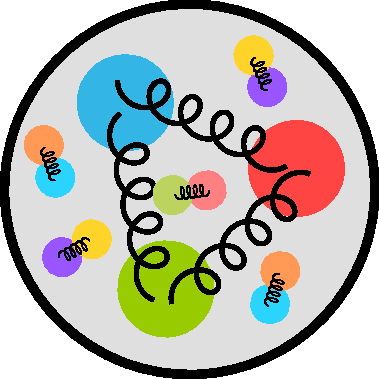
\includegraphics[width=0.5\columnwidth]{proton}
        \end{column}
        \begin{column}{0.05\textwidth}
        \end{column}
    \end{columns}
    \hspace{5.6cm} 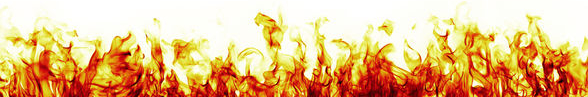
\includegraphics[width=.35\textwidth]{fire}
    \vspace{-.2cm}
    \begin{tcolorbox}[colback=theme!10, colframe=theme!0]
        \centering \large Proton should melt at $\sim$2,000,000,000,000 K!
    \end{tcolorbox}
\end{frame}


\begin{frame}[t]{QCD predicts new phase of matter}
    \bigskip
    QCD calculations on the lattice find the phase transition at $T \approx 155$~MeV, where nucleons 'melt' to form a plasma of deconfined quarks and gluons dubbed a \emph{quark-gluon plasma}\\[2ex]
    \begin{columns}
        \begin{column}{0.47\textwidth}
            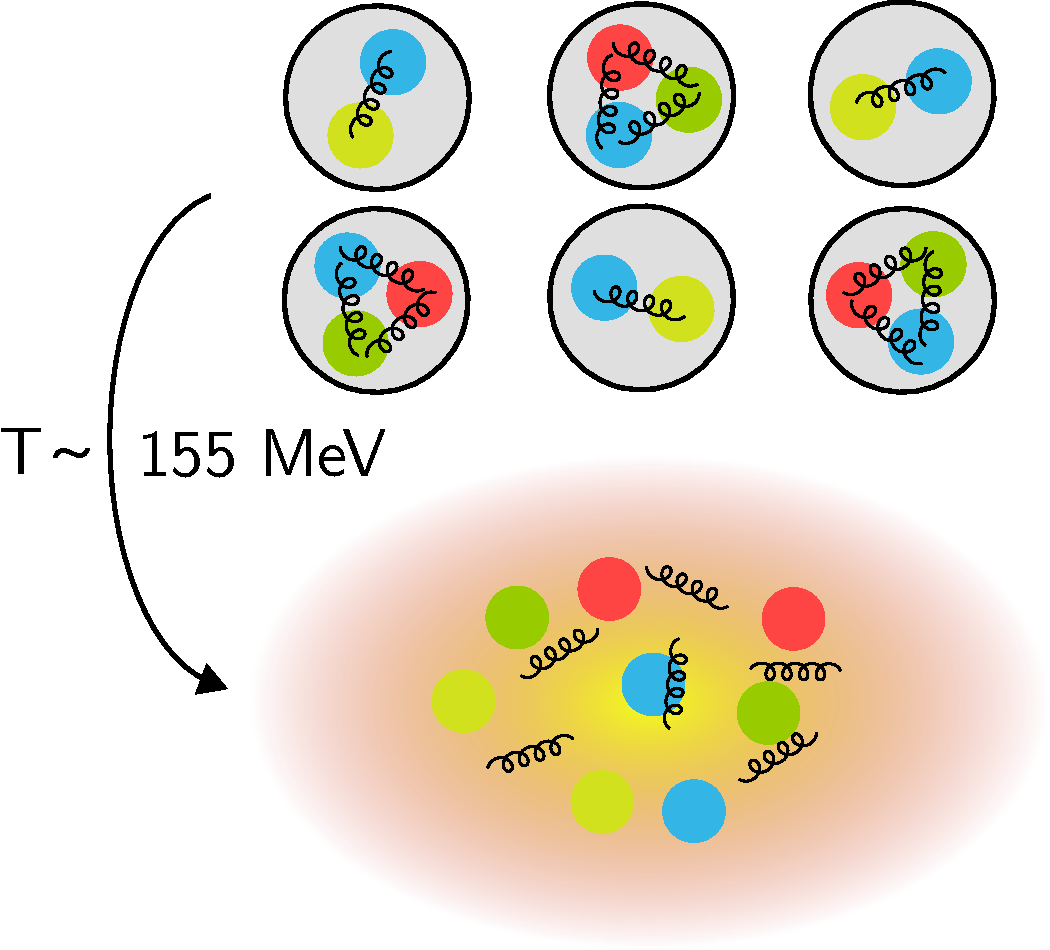
\includegraphics[width=0.8\columnwidth]{confined_deconfined}
        \end{column}
        \begin{column}{0.4\textwidth}
            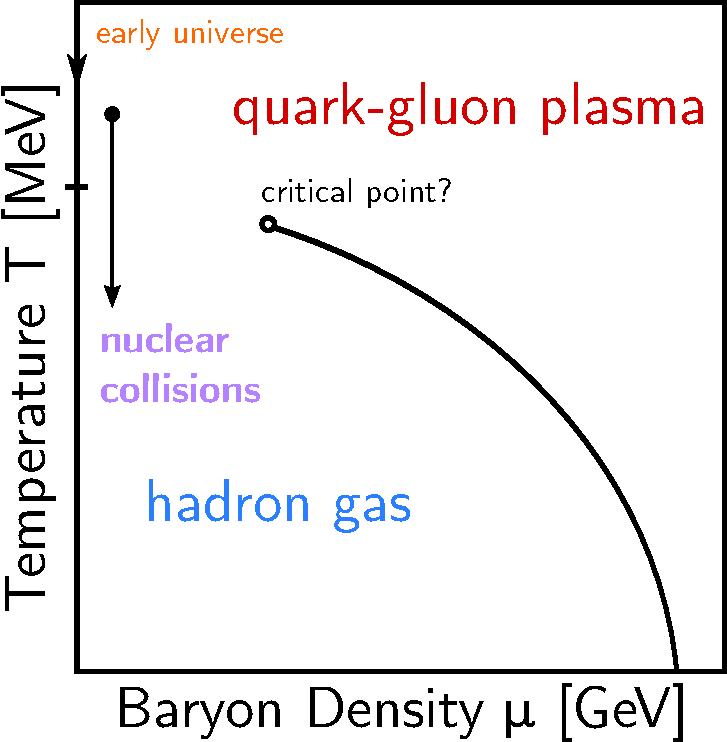
\includegraphics[width=0.8\columnwidth]{phasediagram}
        \end{column}
    \end{columns}
\end{frame}

\begin{frame}[t]{Quark-gluon plasma in nature}
    \bigskip
    Conditions to produce QGP occur(ed) naturally in two places
    \begin{itemize}
        \item Early universe, mere microseconds after big bang where $T > 200$~MeV
        \item Center of neutron stars at extreme baryon density
    \end{itemize}
    \bigskip
    \begin{columns}[T]
    \begin{column}{0.5\textwidth}
        \centering
        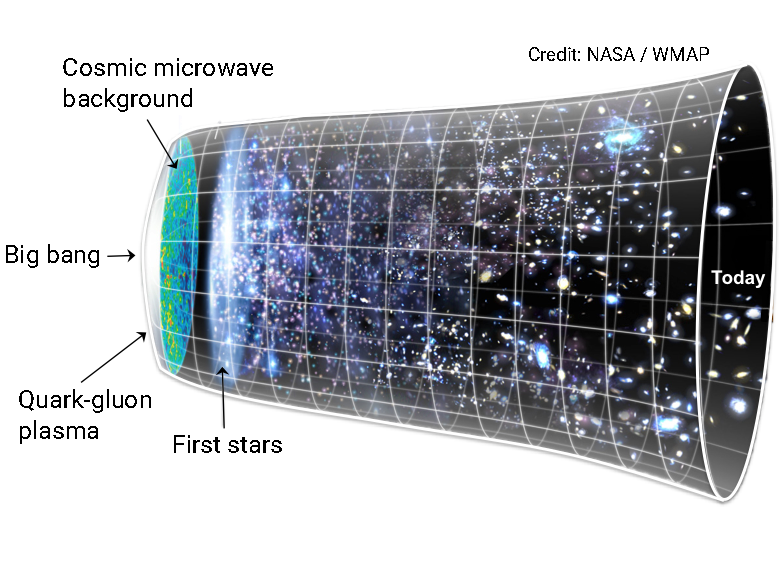
\includegraphics[width=0.9\columnwidth]{bigbang.pdf}
    \end{column}
    \begin{column}{0.5\textwidth}
        \centering
        \bigskip 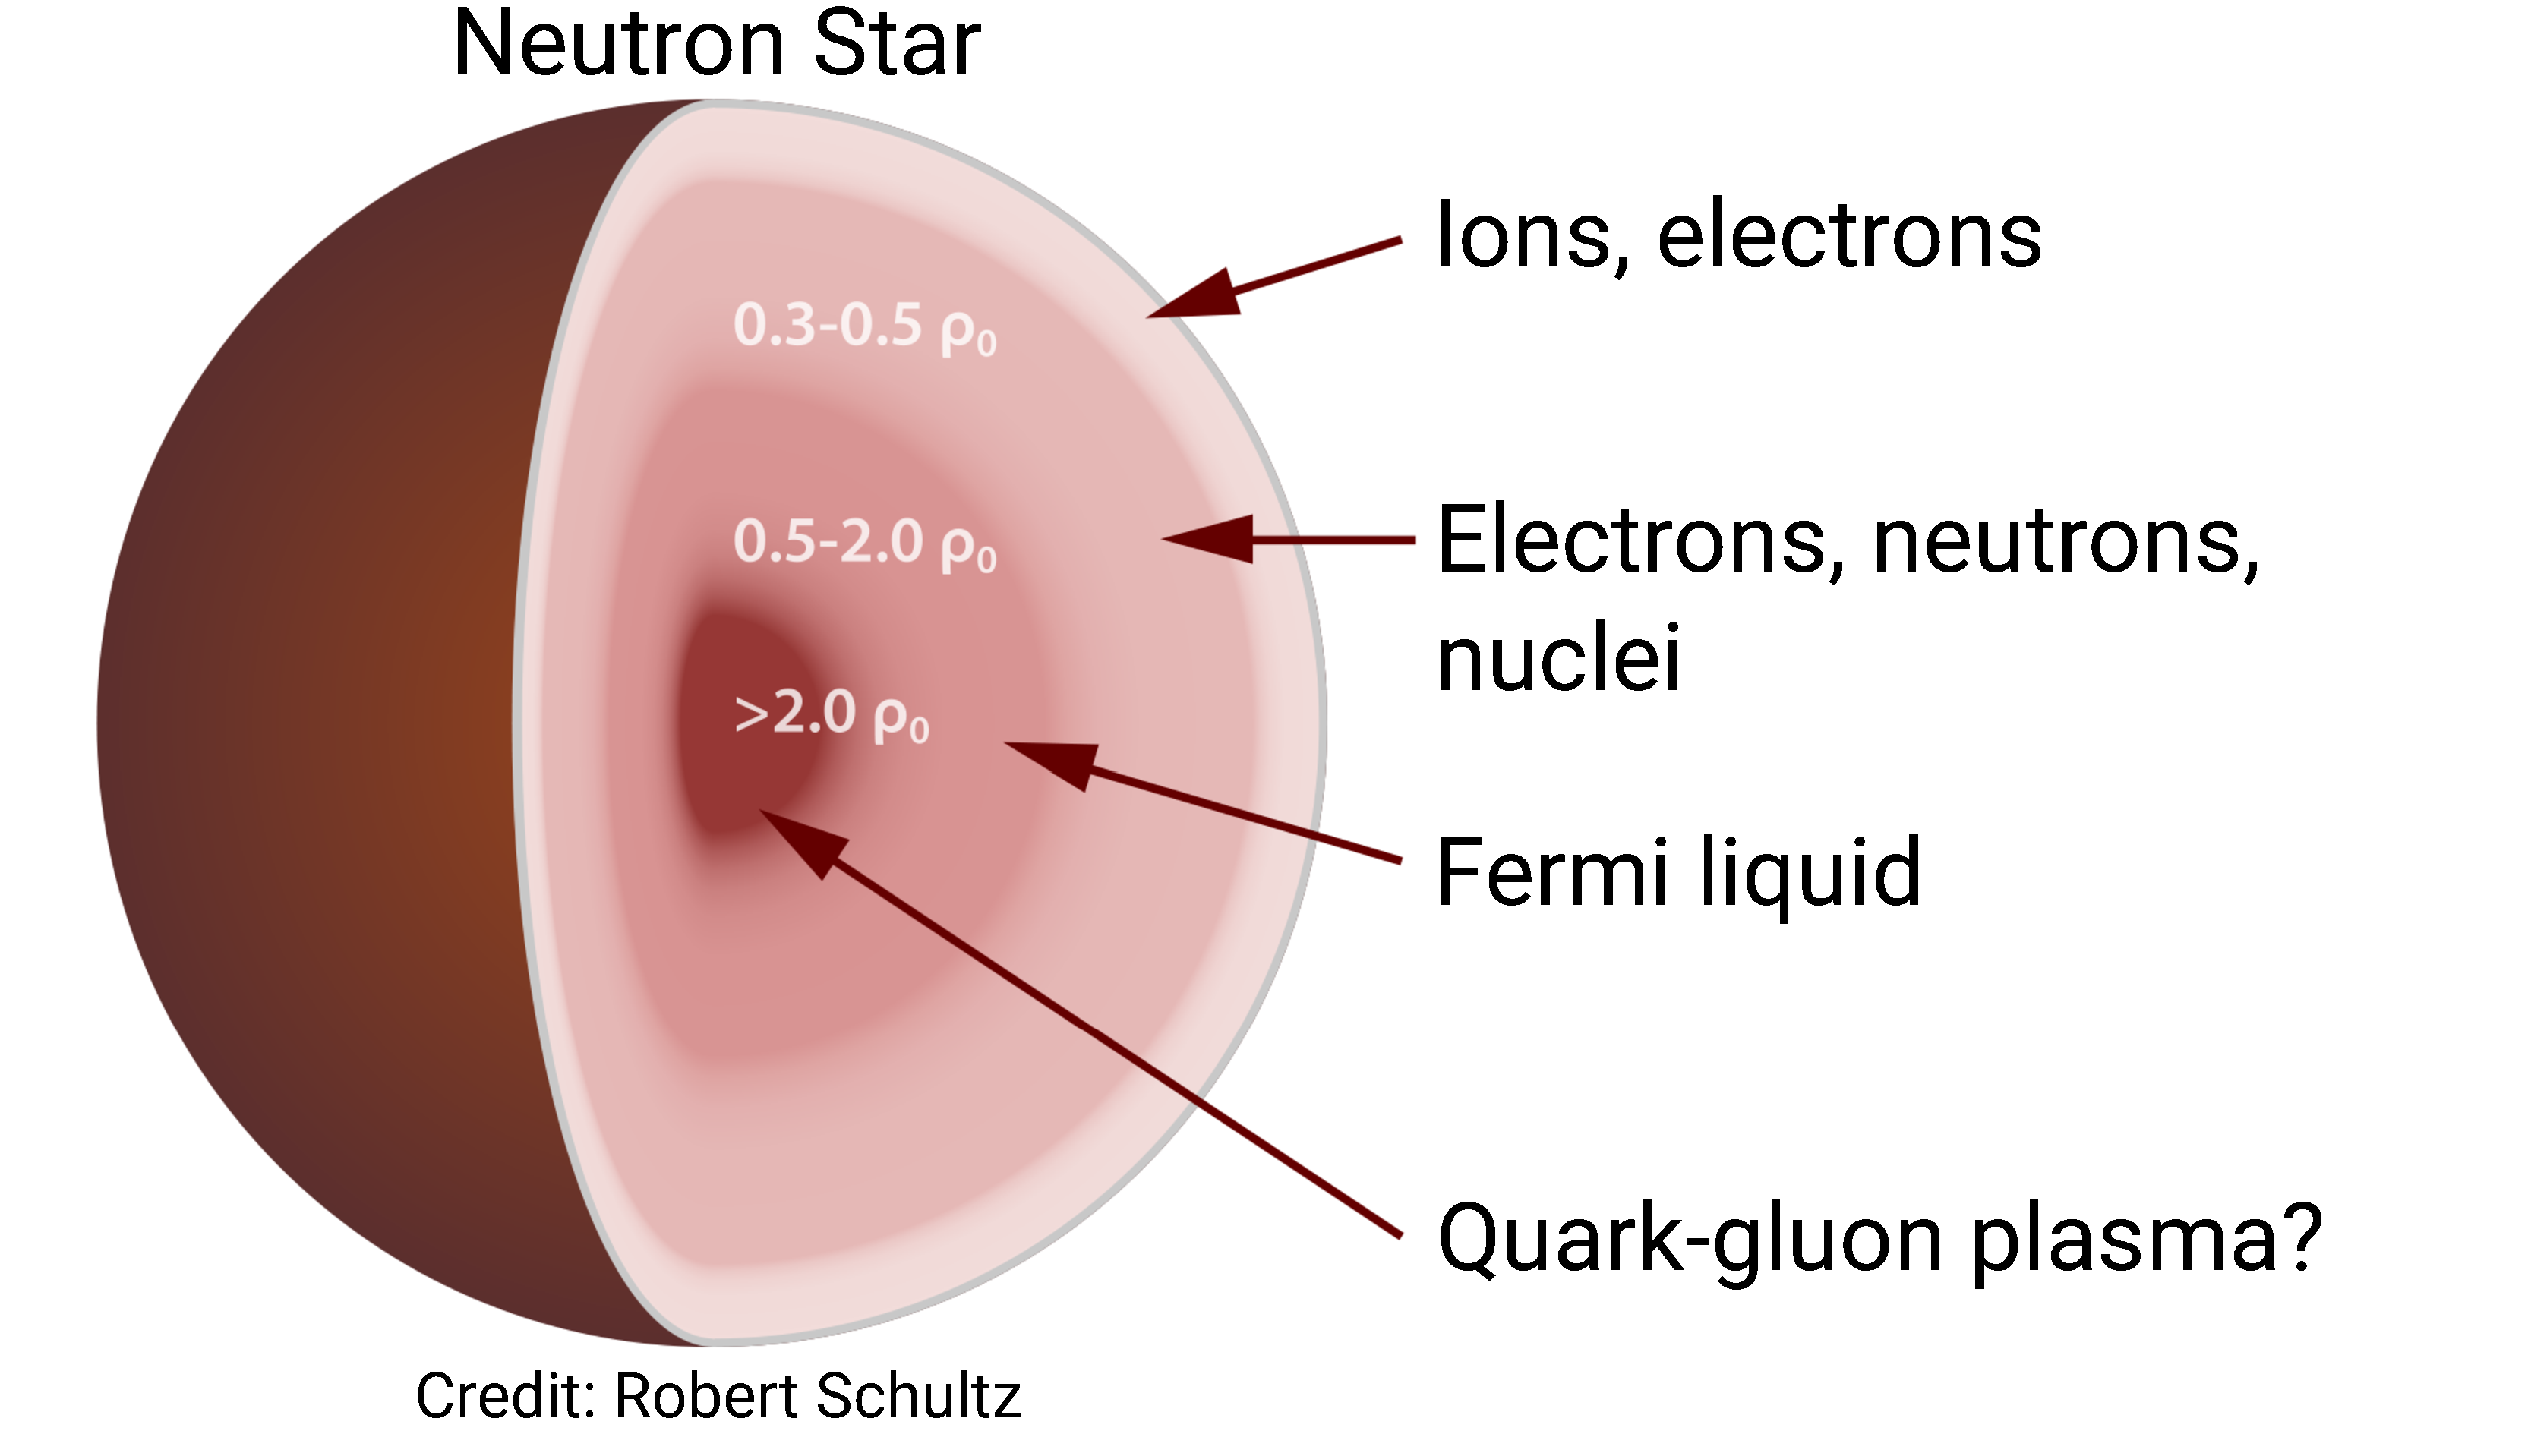
\includegraphics[width=0.9\columnwidth]{neutronstar.pdf}
    \end{column}
    \end{columns}
\end{frame}


\begin{frame}[t]{Creating quark-gluon plasma in the laboratory}
\bigskip
General strategy... collide nuclei at ultrarelativistic energies
\medskip
\begin{itemize}
    \item Relativistic Heavy-ion Collider (RHIC):\\
          Beam energy 7.7--200~GeV per nucleon pair
    \item Large Hadron Collider (LHC):\\
          Beam energy 2760--13000~GeV per nucleon pair
\end{itemize}
\vspace{-.3cm}
\begin{columns}[T]
    \begin{column}{0.05\textwidth}
    \end{column}
    \begin{column}{0.9\textwidth}
        \only<1>{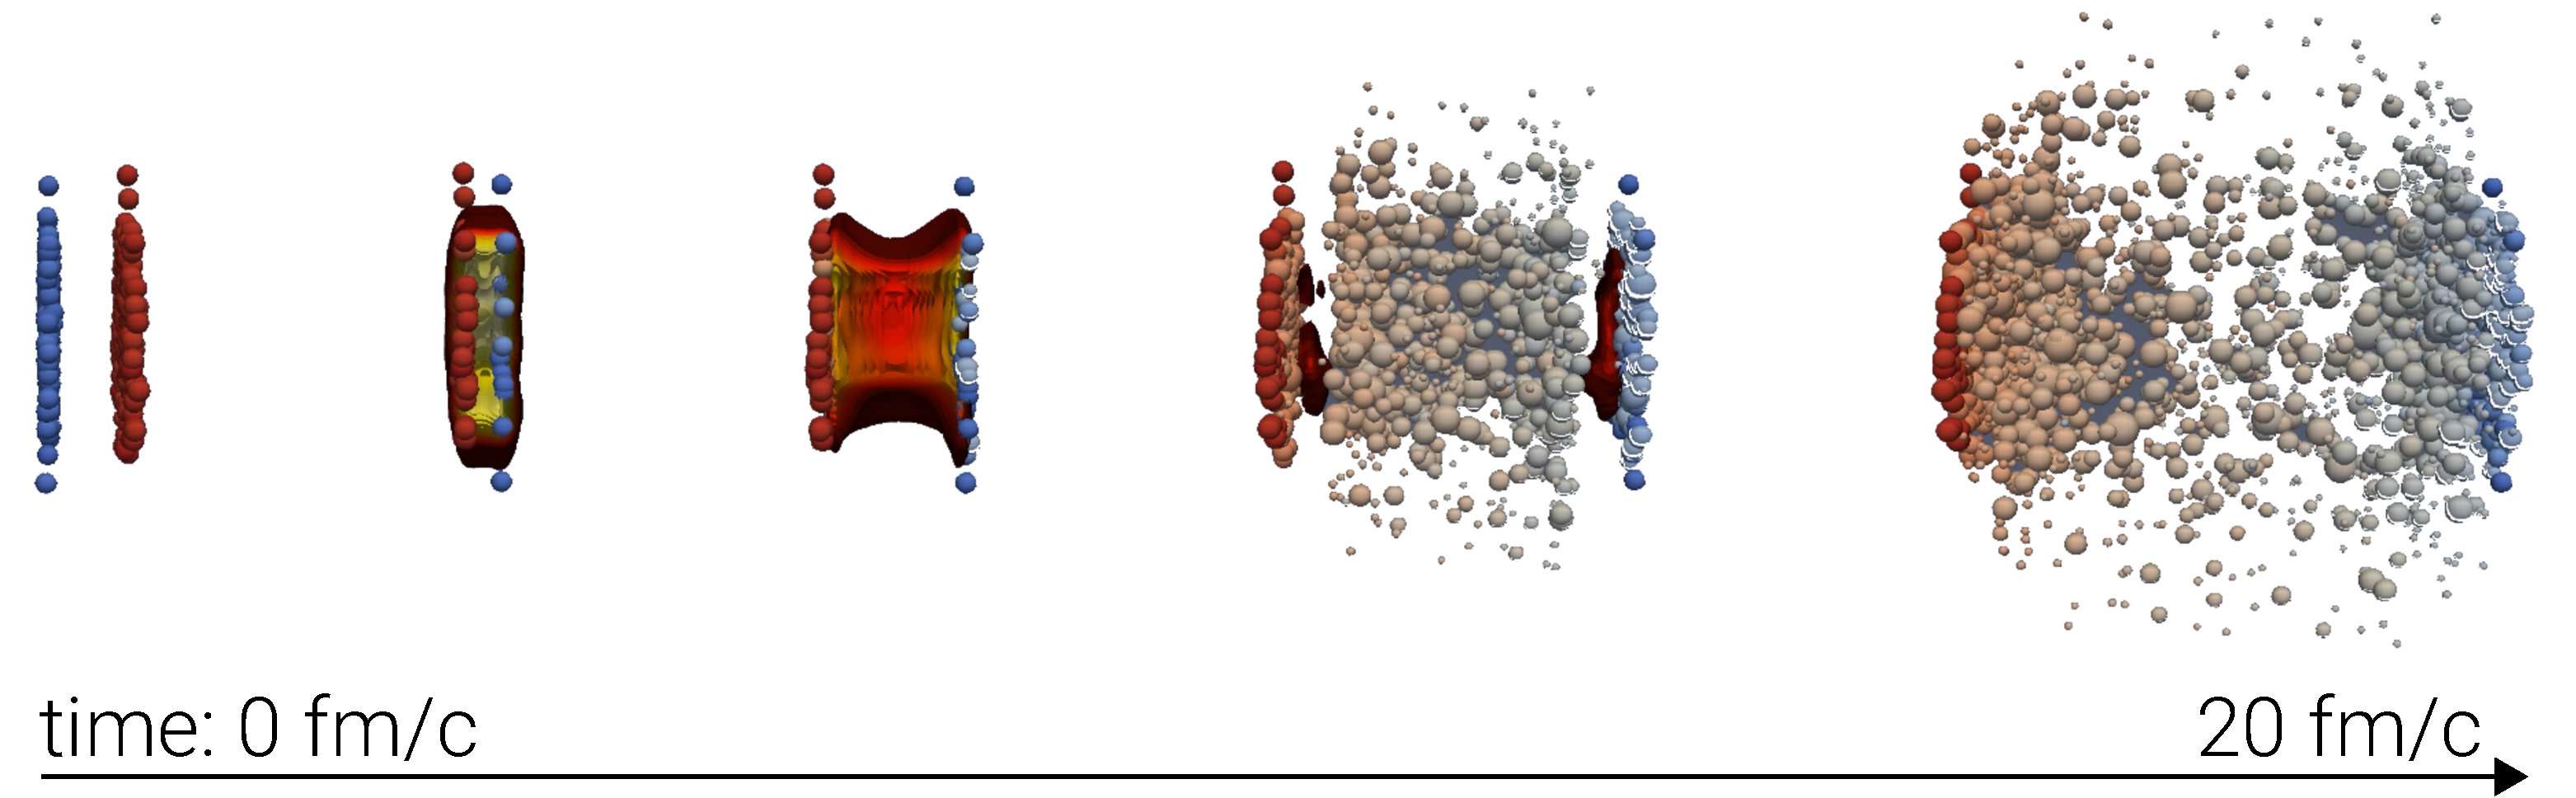
\includegraphics[width=\textwidth]{hic_picture1}\\
                 {\scriptsize \hspace{0.12cm} Fig.\ MADAI collaboration}}
        \only<2>{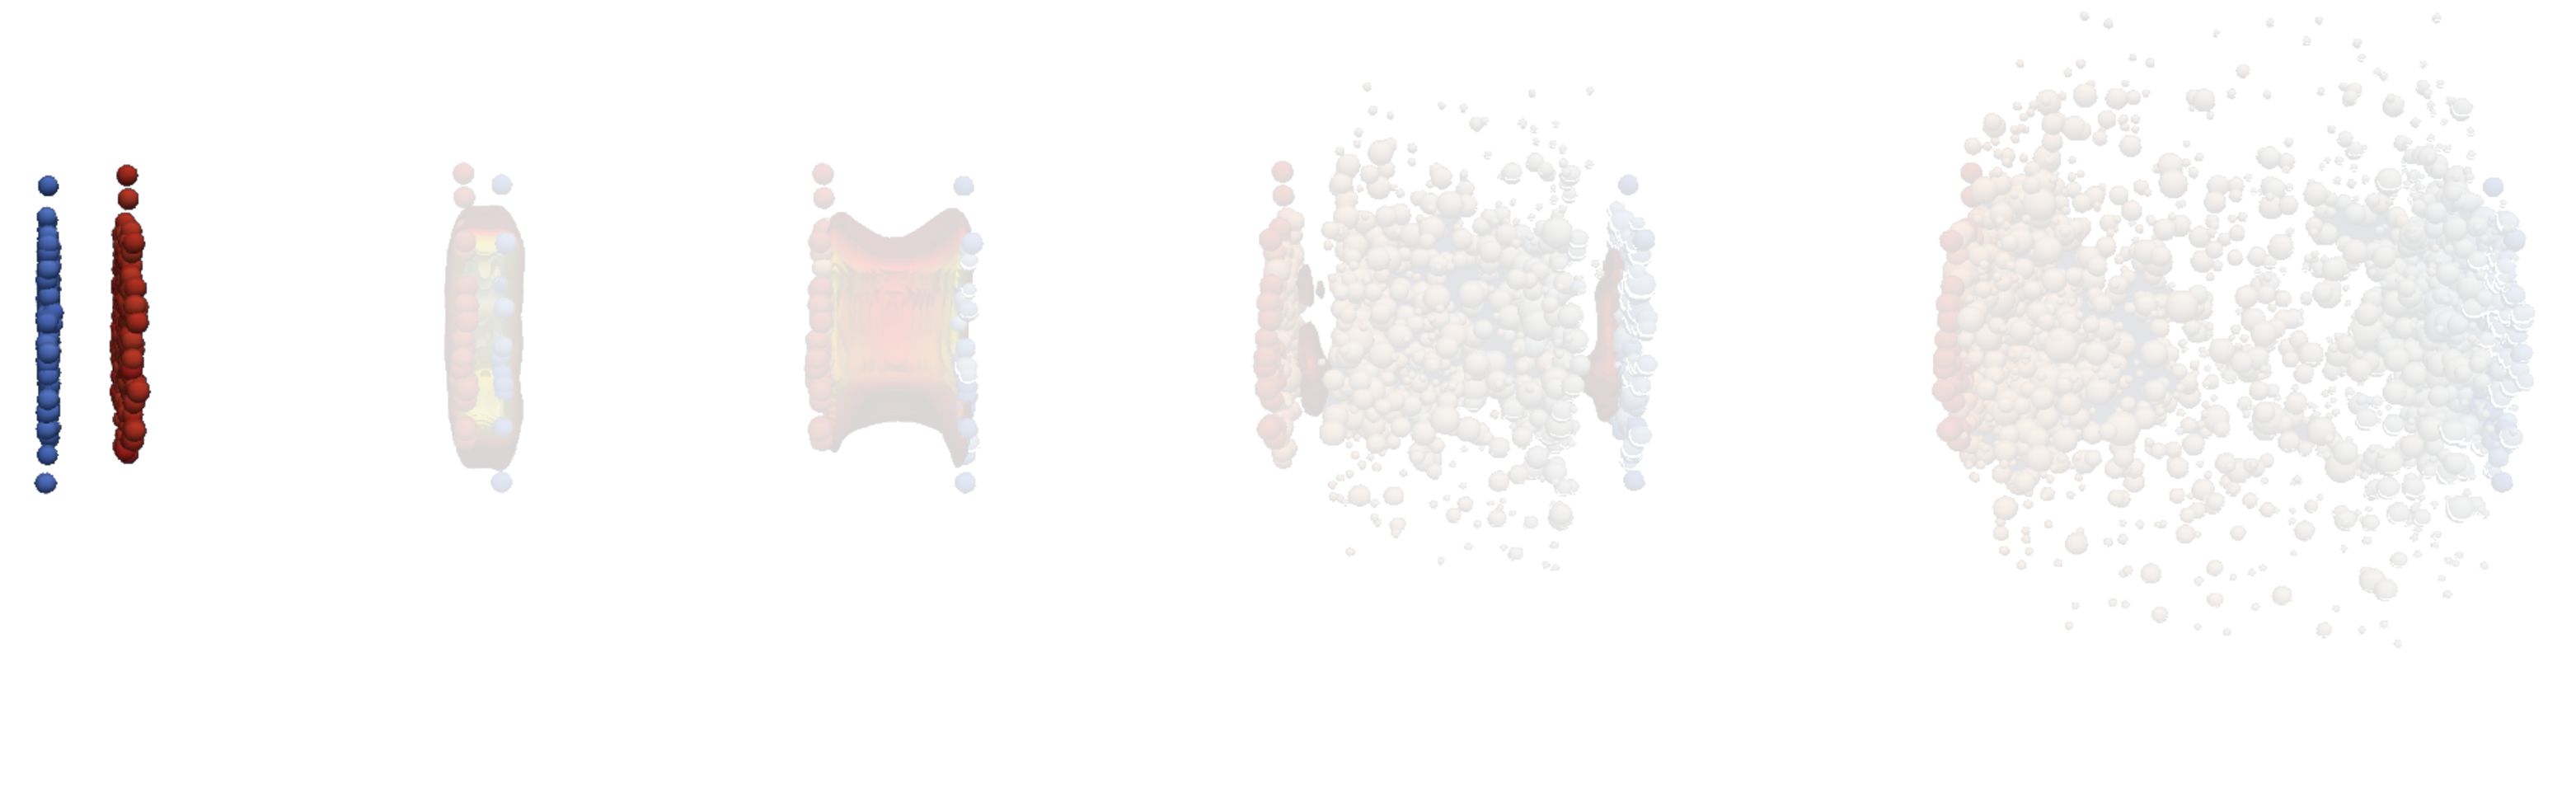
\includegraphics[width=\textwidth]{hic_picture2}\\
                 \centering \vspace{-.8cm}
                 Relativistic nuclei highly Lorentz contracted
                 ...pancake-shaped in lab frame} 
        \only<3>{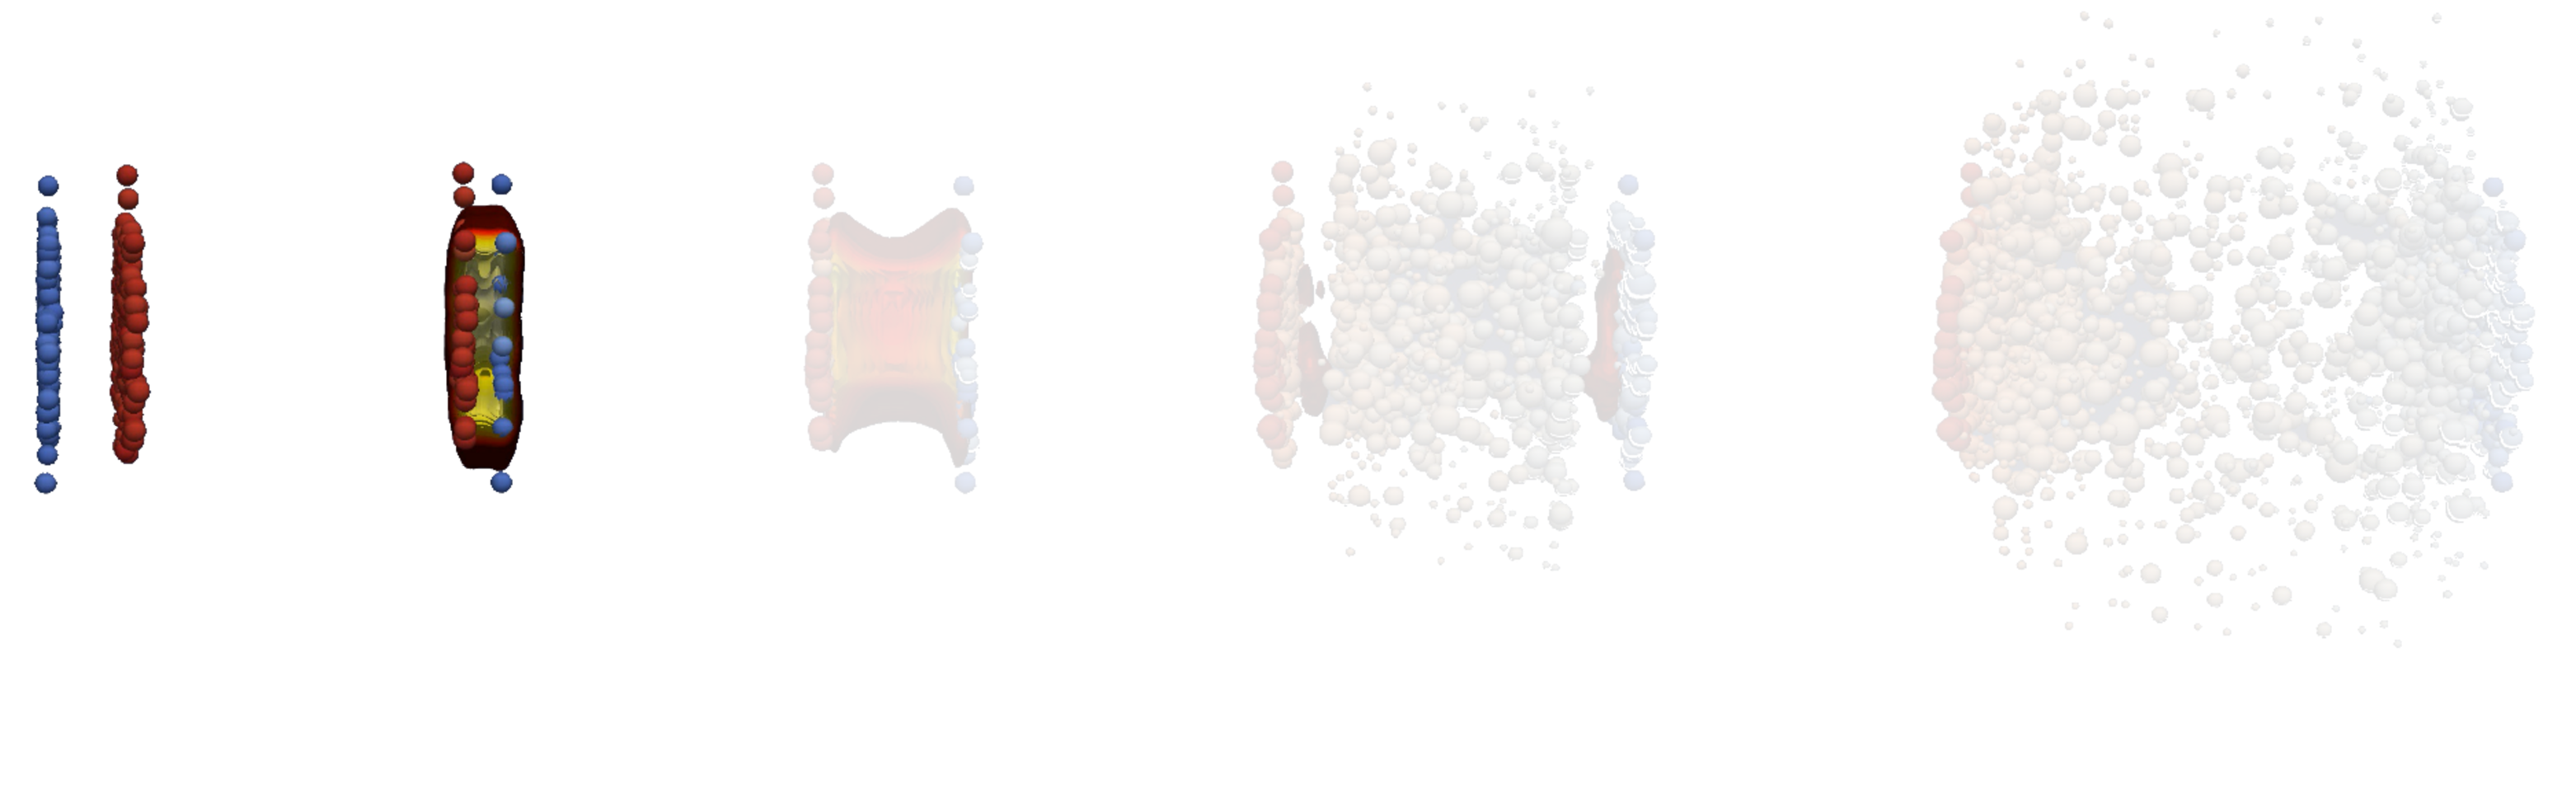
\includegraphics[width=\textwidth]{hic_picture3}\\
                 \centering \vspace{-.8cm}
                 Nuclei collide, compress and heat matter beyond QGP critical point}
        \only<4>{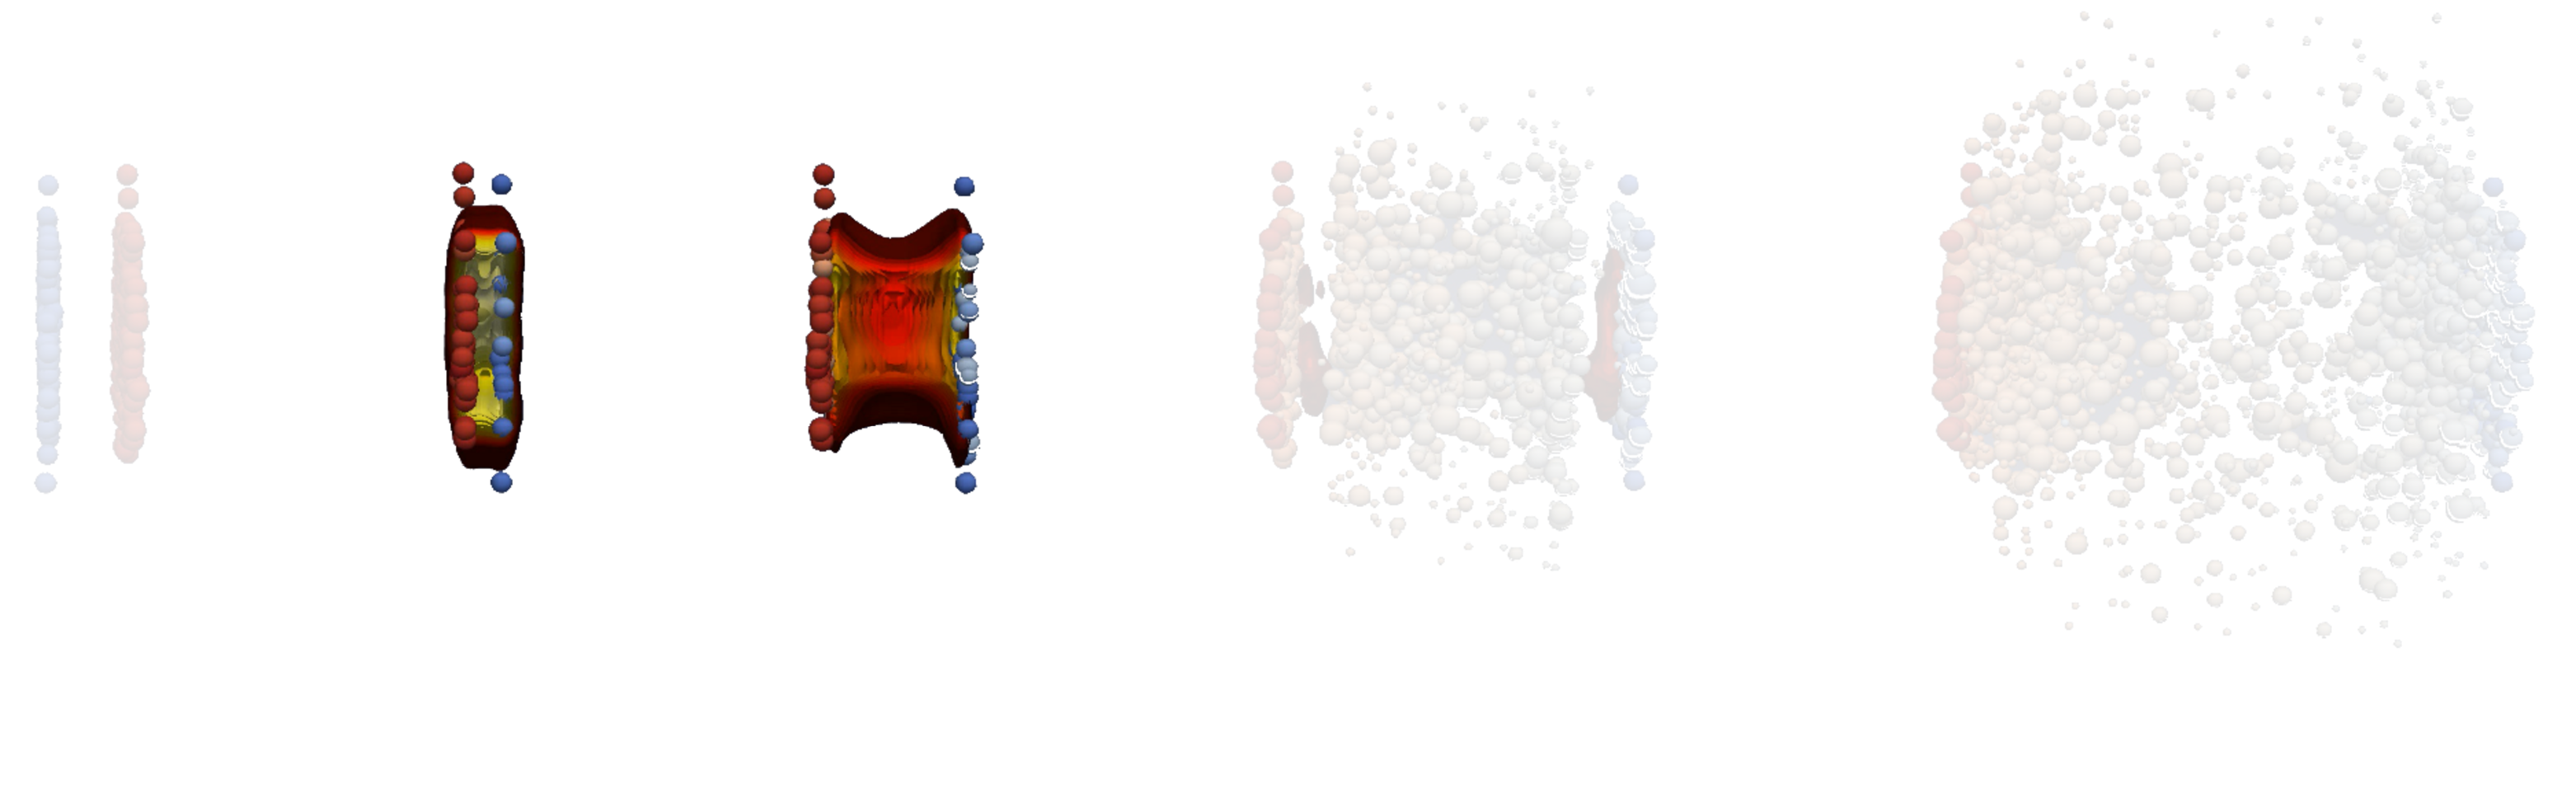
\includegraphics[width=\textwidth]{hic_picture4}
                 \centering \vspace{-.8cm}
                 QGP thermalizes, starts to expand hydrodynamically
                }
        \only<5>{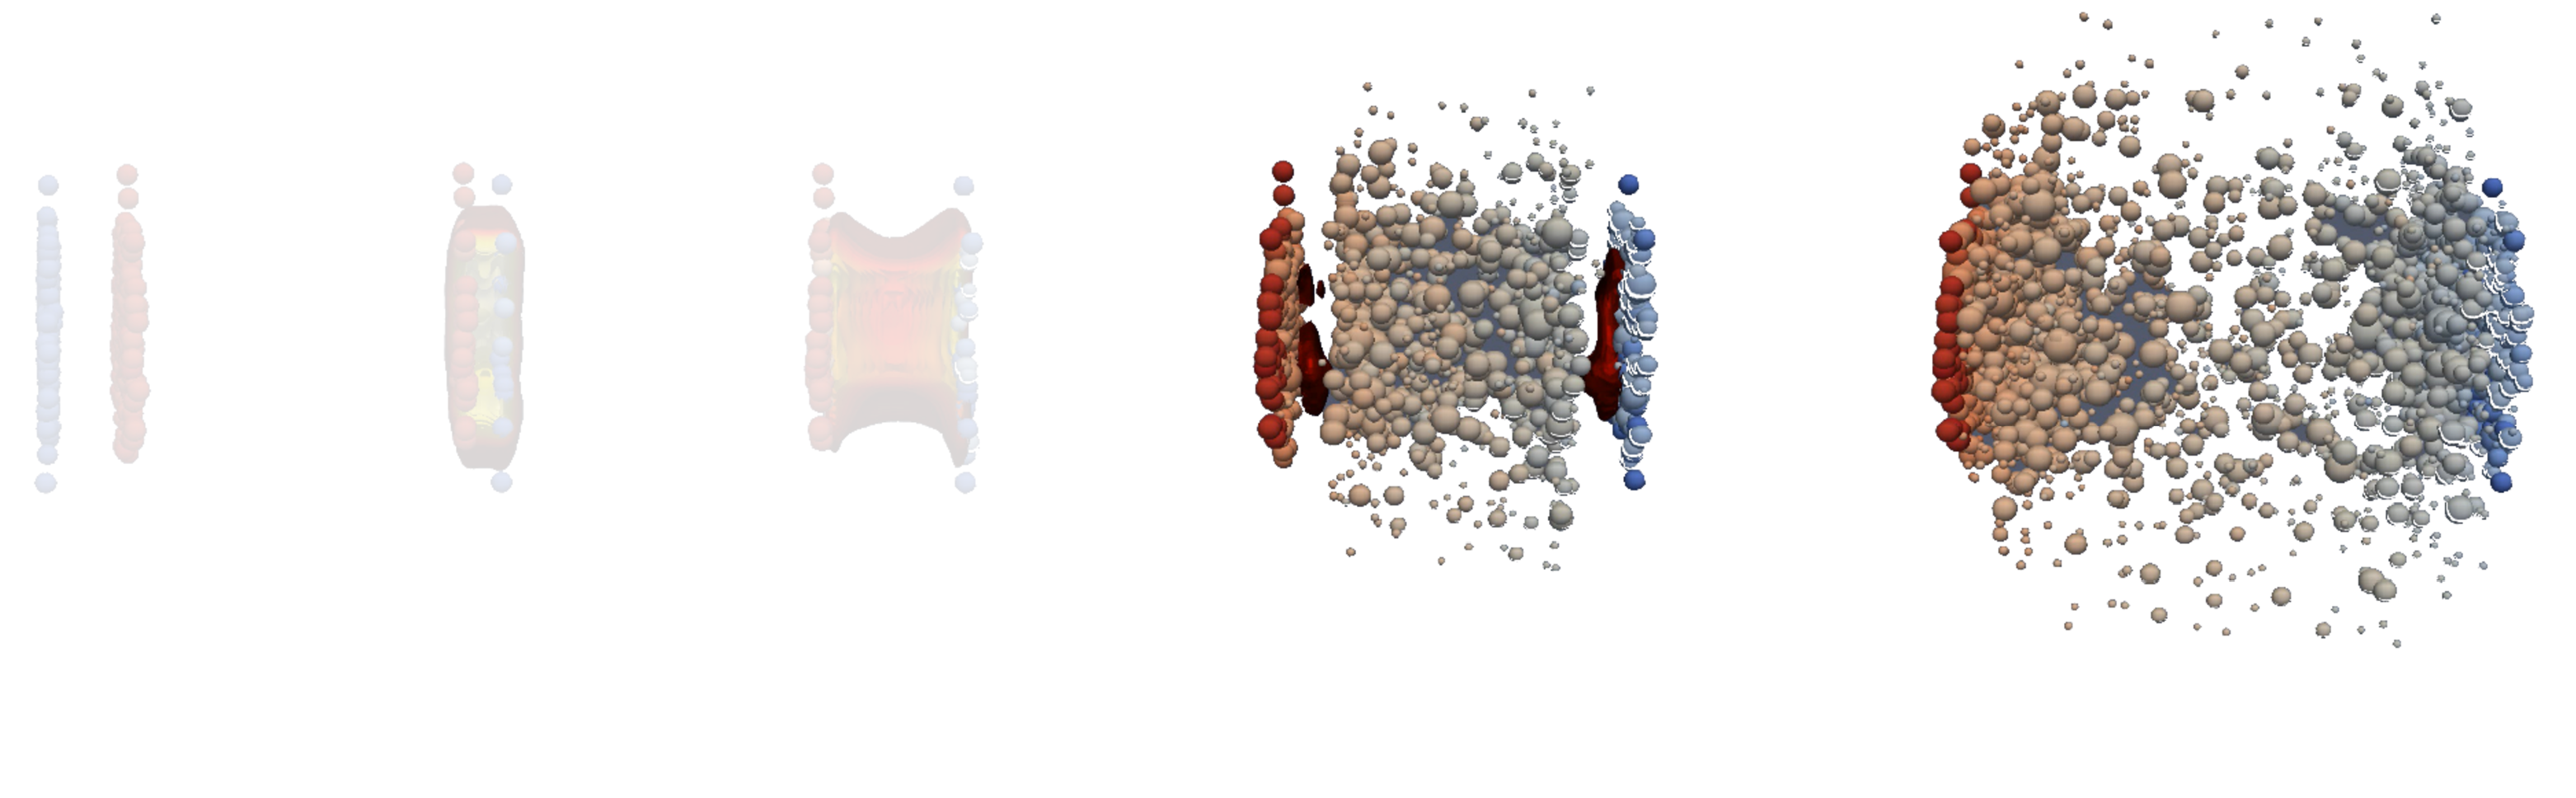
\includegraphics[width=\textwidth]{hic_picture5}
                 \centering \vspace{-.8cm}
                 Quarks and gluons recombine into colorless hadrons and hit the detector.
                }
    \end{column}
    \begin{column}{0.05\textwidth}
    \end{column}
\end{columns}
\end{frame}


\begin{frame}{Studying bulk properties of the QGP liquid}
    \begin{center}
        \begin{tikzpicture}
            \node[anchor=center, xshift=1cm, yshift=0.75cm] (qgp) at (current page.center) {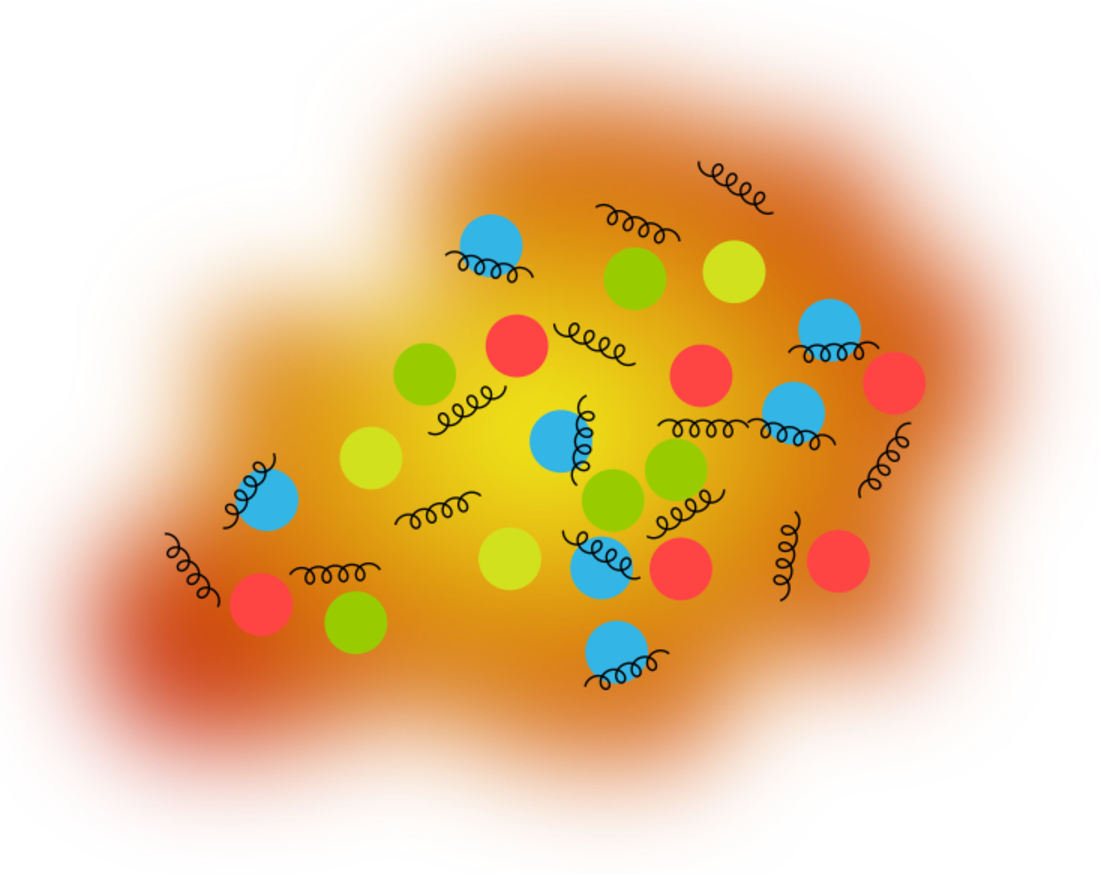
\includegraphics[width=0.35\textwidth]{qgp}};
            \node[text width=4cm, xshift=6cm, yshift=3cm] (t1) at (current page.center) {How and under what\\ conditions is it formed\\ in a nuclear collision?};
            \node[text width=4.75cm, xshift=6.5cm, yshift=-1.5cm] (t2) at (current page.center) {How does it recombine\\ to form colorless hadrons?};
            \node[text width=4cm, xshift=-2.5cm, yshift=3cm] (t3) at (current page.center) {Equation of state?\\ Relations between\\ thermal quantities,\\ e.g.\ $P=P(\epsilon)$};
            \node[text width=4cm, xshift=-3.5cm, yshift=-2cm] (t4) at (current page.center) {Transport properties?\\ shear/bulk viscosity,\\ probe energy loss, etc};
            \path[->, >=stealth, theme] ([xshift=-.1cm]t1.west) edge [out=-180, in=90] (qgp.north);
            \path[->, >=stealth, theme] ([yshift=.1cm]t2.north) edge [out=90, in=-30] (qgp.east);
            \path[->, >=stealth, theme] ([xshift=-.8cm]t3.south) edge [out=-90, in=180] (qgp.west);
            \path[->, >=stealth, theme] (t4.east) edge [out=0, in=-90] (qgp.south);
        \end{tikzpicture}
    \end{center}
\end{frame}

\begin{frame}{Quark-gluon plasma is not directly detectable}
    \medskip
    \centering
    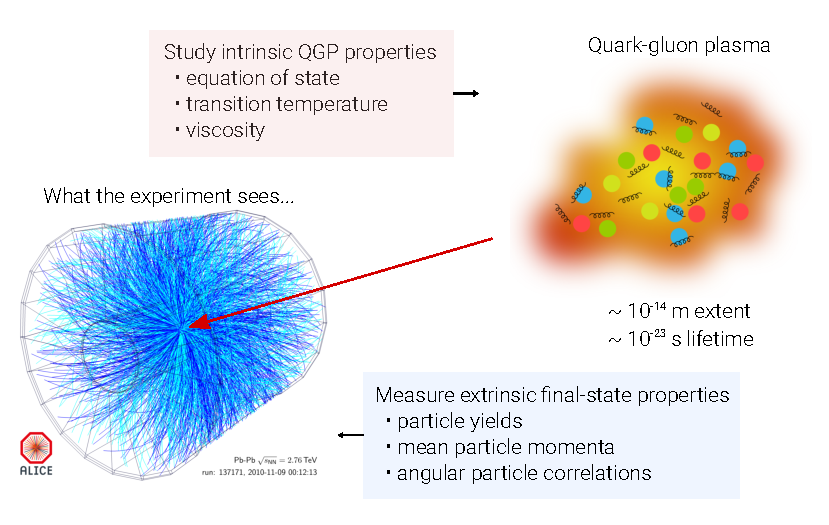
\includegraphics[height=0.85\textheight]{qgp_modeling}
\end{frame}

\begin{frame}[t, plain]{Notable example: infer viscosity from flow anisotropy}
\only<1>{
    \vspace{0.2cm}
    \begin{columns}
        \begin{column}{0.025\textwidth}
        \end{column}
        \begin{column}{0.475\textwidth}
            \centering
            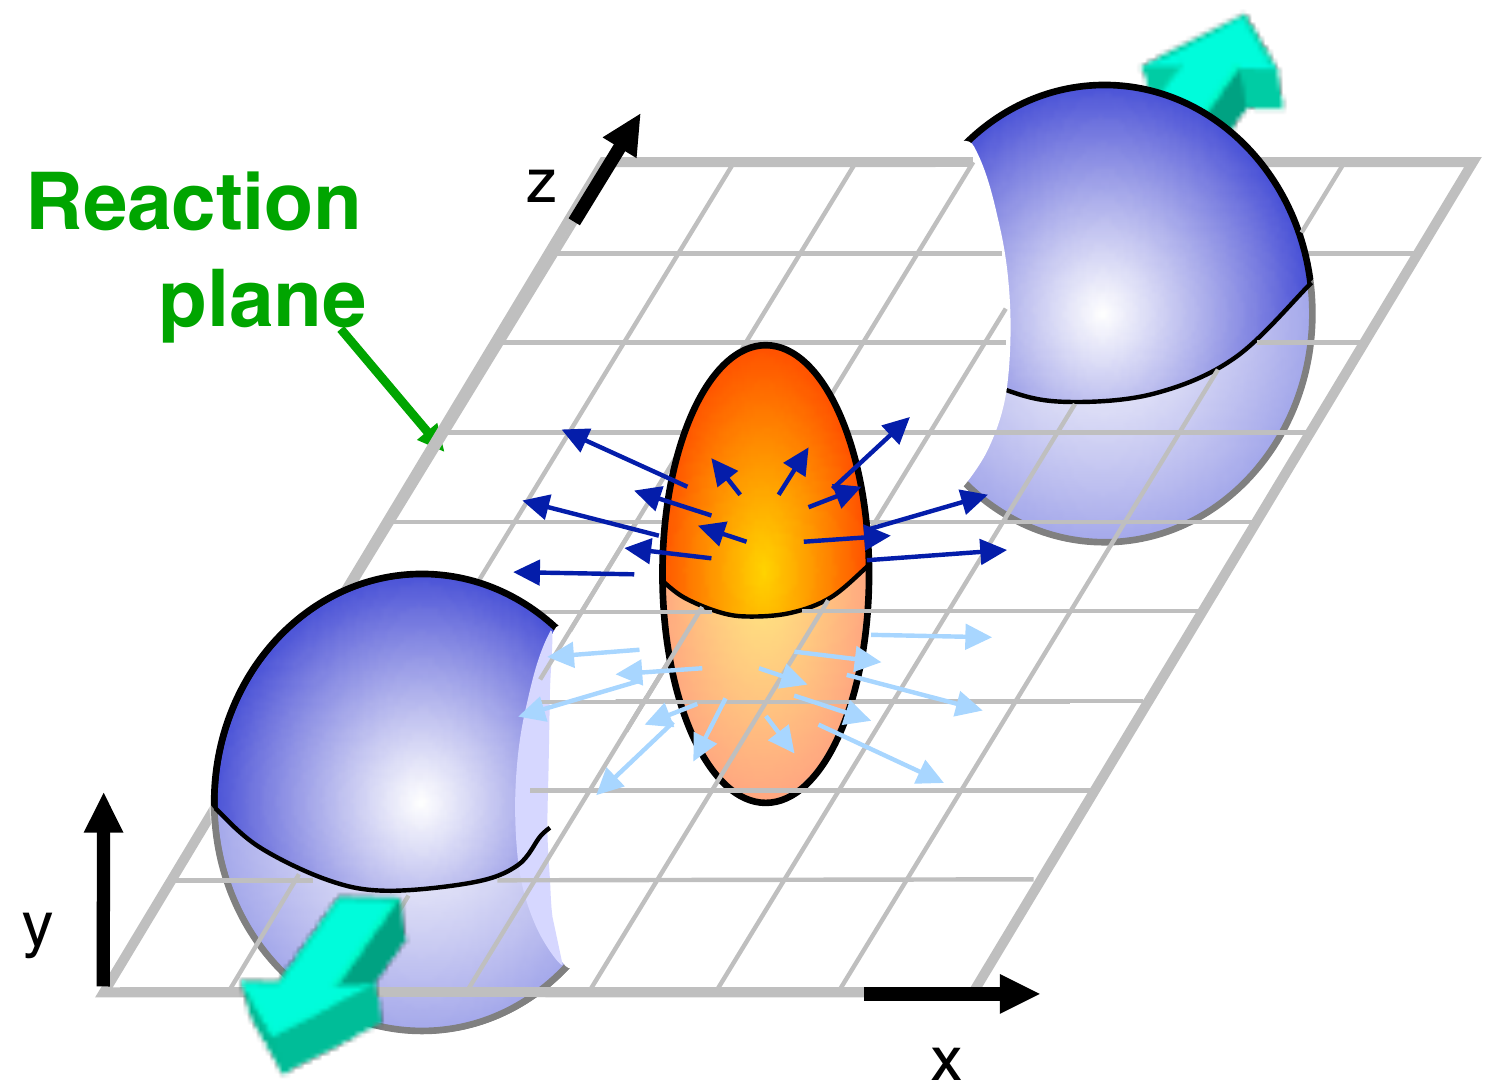
\includegraphics[width=0.65\textwidth]{collision_geometry}
        \end{column}
        \begin{column}{0.475\textwidth}
            \centering
            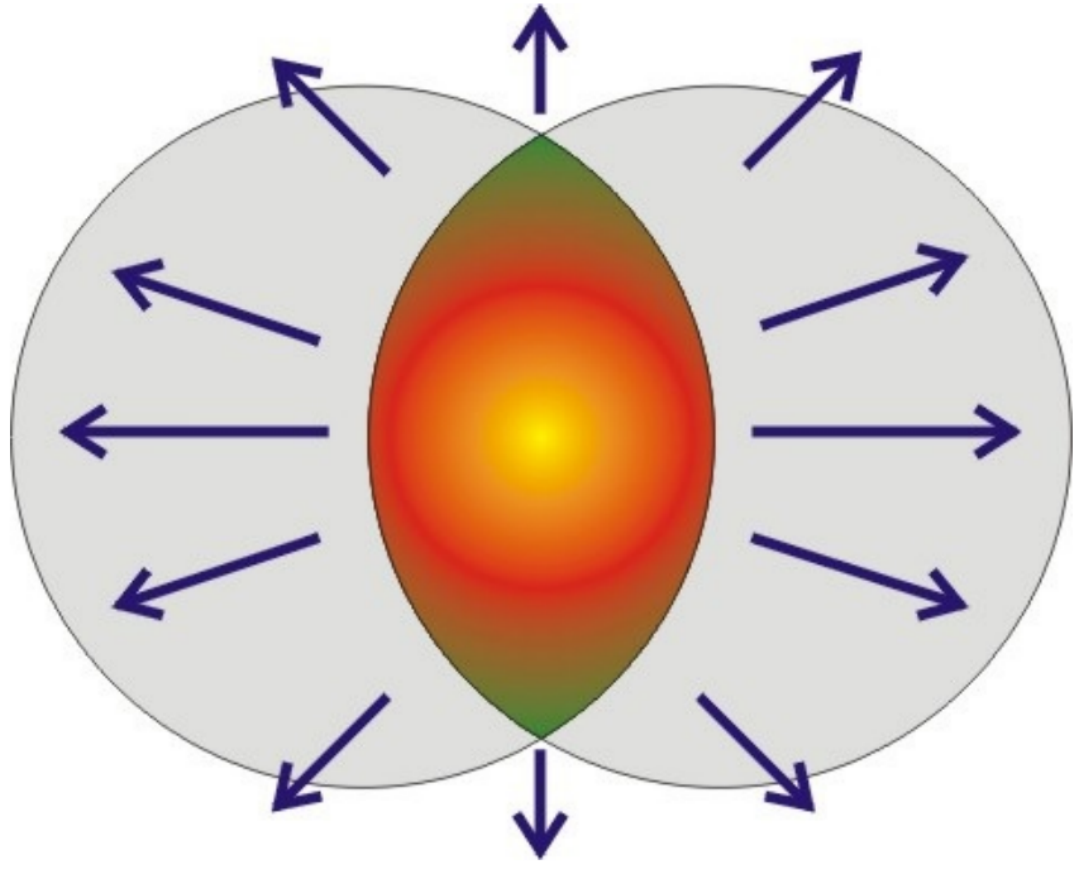
\includegraphics[width=0.45\textwidth]{overlap}\\
            \small Overlap region, compressed and heated
        \end{column}
        \begin{column}{0.025\textwidth}
        \end{column}
    \end{columns}
    \medskip \hrule \bigskip
    \begin{columns}[T]
        \begin{column}{0.025\textwidth}
        \end{column}
        \begin{column}{0.5\textwidth}
            \medskip
            \small Elliptic flow ($v_2$):
            \begin{itemize}
                \small
                \item pressure gradients steeper along short axis of ellipse, drives asymmetric flow\\
                \item quantified by 2$^\mathrm{nd}$ Fourier coeff. of angular dist: $v_2$\\
                \item Good agreement for small viscosity $\eta/s$
            \end{itemize}
        \end{column}
        \begin{column}{0.45\textwidth}
            \centering
            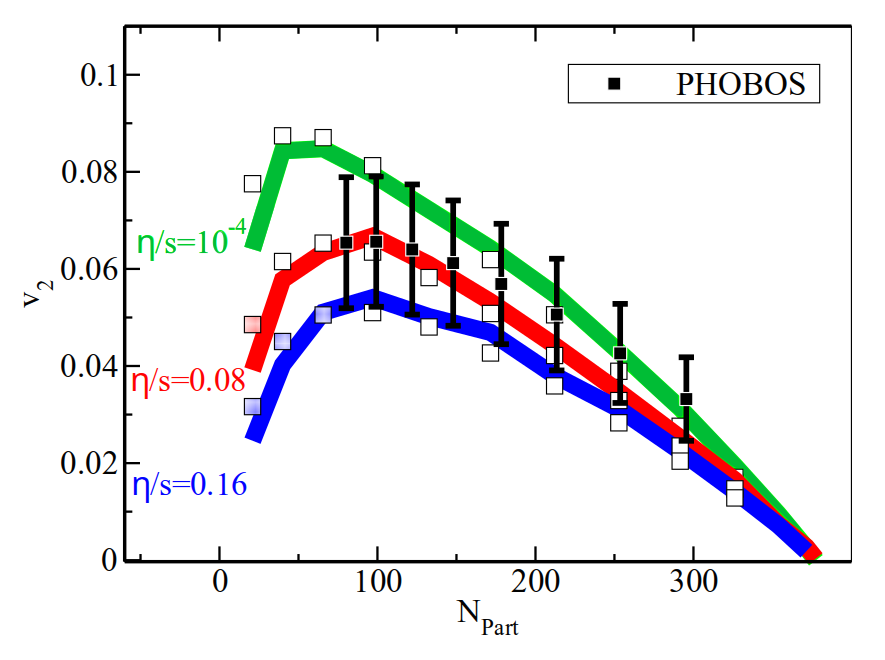
\includegraphics[width=0.75\textwidth]{v2}\\
            \scriptsize Fig.\ credit: Luzum, Romatschke
        \end{column}
        \begin{column}{0.025\textwidth}
        \end{column}
    \end{columns}}
\only<2>{
    \centering \vspace{0.6 cm}
    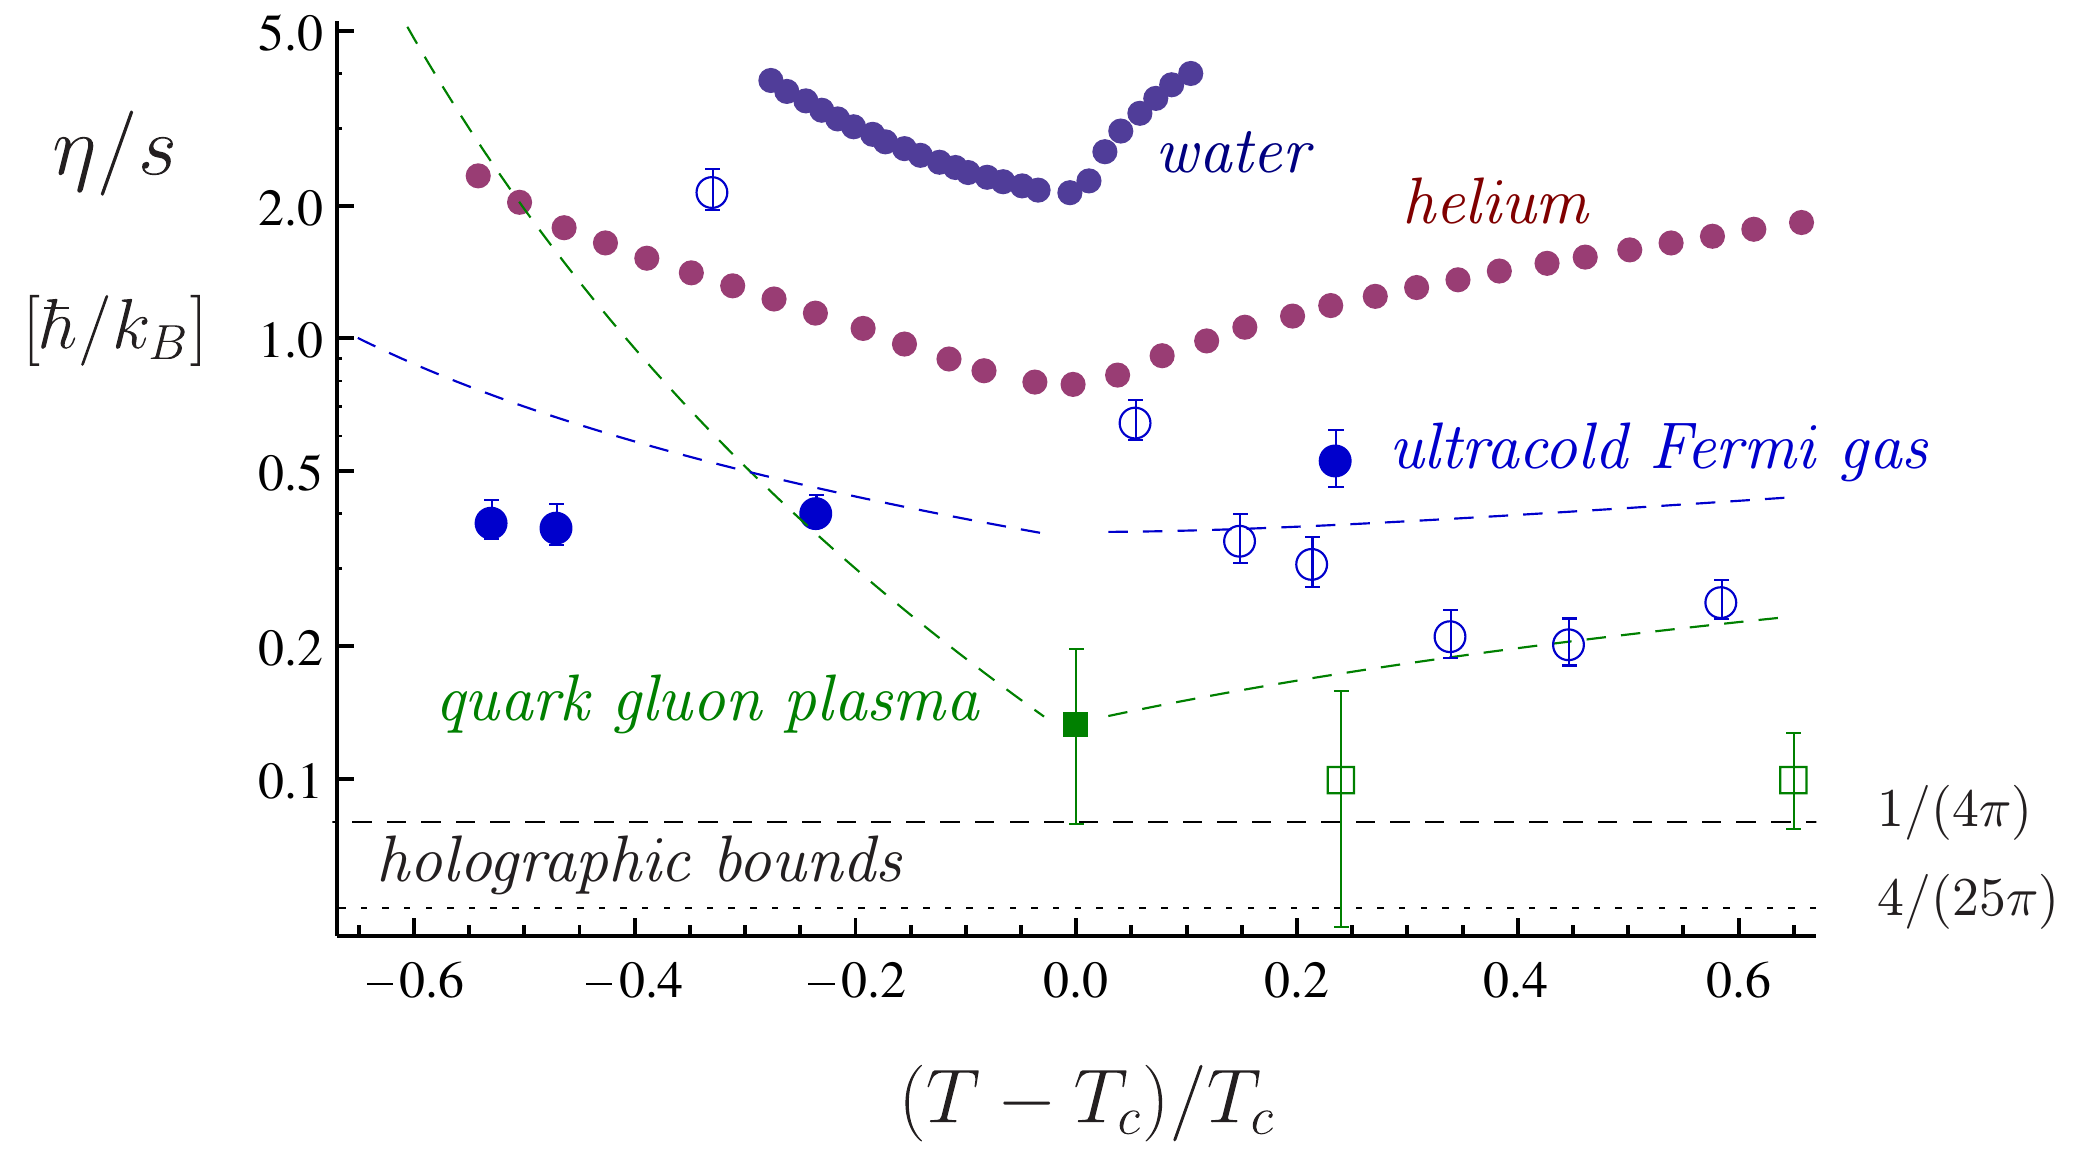
\includegraphics[width=0.7\textwidth]{eta-bound}\\
    {\scriptsize A.\ Adams, et.\ al.\ New Journal of Physics 14 (2012)}\\[1ex]
    \textcolor{theme}{QGP believed to be most ideal fluid in nature!}
}
\end{frame}


\begin{frame}[plain]{Transport models connect experiment and theory}
    \bigskip
    \begin{columns}[T]
        \begin{column}{0.05\textwidth}
        \end{column}
        
        \begin{column}{0.4\textwidth}
            \bigskip
            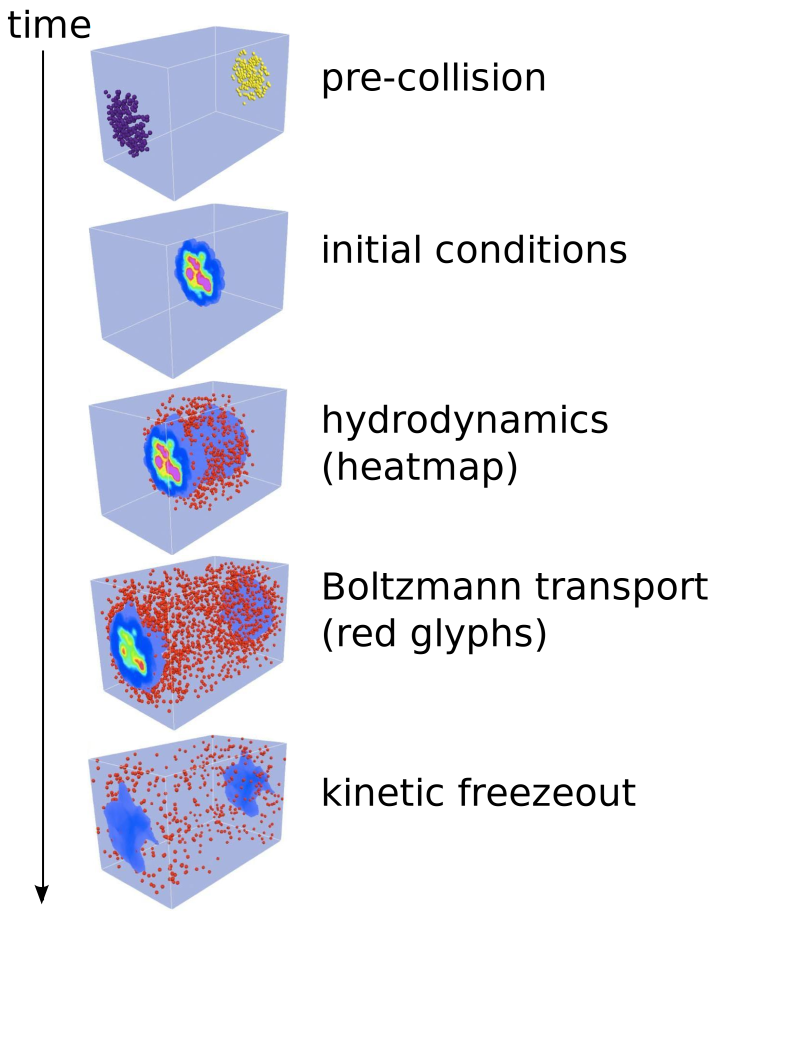
\includegraphics[height=0.9\textheight]{evolution}
        \end{column}
        
        \begin{column}{0.5\textwidth}
            \bigskip
            \begin{block}{\strut \small Initial conditions}
                \footnotesize
                \textcolor{almostblack}{
                Describe initial $T^{\mu\nu}$ 
                at the QGP thermalization time}
            \end{block}
      
            \begin{block}{\strut \small Hydrodynamics (QGP)}
                \footnotesize
                \textcolor{almostblack}{
                Hydrodynamics imposes energy\\and momentum conservation,\\[1ex] 
                \quad $\displaystyle \partial_\mu T^{\mu \nu} = 0$\\[1ex]
                Requires medium viscosity and equation of state from LQCD}
            \end{block}

            \begin{block}{\strut \small Boltzmann Eqn (hadron gas)}
                \footnotesize
                \textcolor{almostblack}{
                Fluid discretized into particles at transition temperature.\\[1ex]
                Non-equillibrium Boltz. transport,\\[1ex]
                \quad $\displaystyle \frac{df_i(x,p)}{dt} = \mathcal{C}_i(x,p)$}
            \end{block}
        \end{column}
        
        \begin{column}{0.05\textwidth}
        \end{column}
    \end{columns}
\end{frame}


\begin{frame}[t]{Model-to-data comparison: solving the inverse problem}
    \centering \bigskip
    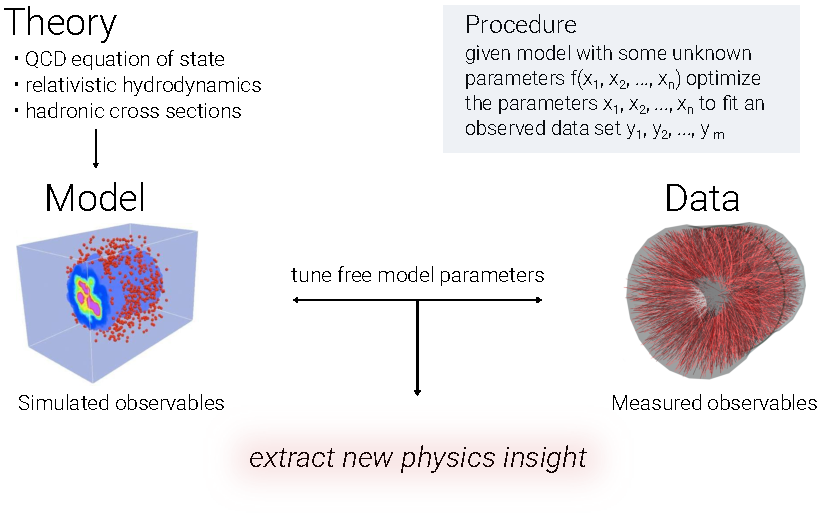
\includegraphics[height=0.85\textheight]{model2data}
\end{frame}


\begin{frame}{Current practicum and thesis work}
    \hspace{2cm} \medskip
    \emph{\quad "What are you doing and why are you doing it." \\ \hspace{9.5 cm}--sponsors}
    \bigskip
    \setbeamercovered{transparent}
    \begin{columns}
    \begin{column}{0.8\textwidth}
    \begin{enumerate}
        \onslide<1,2>{\item Quantify sensitivity of hydrodynamic simulations to different\\ 
              calculations of the QCD equation of state (LLNL)\\
              {\scriptsize Phys.\ Rev.\ C93 (2016) 044913}\\[1ex]}
        \onslide<1>{\item Improve theoretical description of the QGP initial conditions\\
              {\scriptsize Nucl.\ Phys.\ A 904-905, 815c (2013)}\\
              {\scriptsize Phys.\ Rev.\ C92 (2015) 011901}\\[1ex]}
        \onslide<1>{\item Rigorously constrain QGP medium properties using\\ Bayesian model-to-data analysis\\
              {\scriptsize pre-print\, arXiv:1605.03954 (2016)}}
    \end{enumerate}
    \end{column}
    \end{columns}
\end{frame}


\begin{frame}{Studying the QGP equation of state}
    \vspace{0.6 cm}
    Equation of state calculable from QCD Lagrangian $\mathcal{L}[A_\mu^a,\bar\Psi, \Psi]$\\[1ex]
    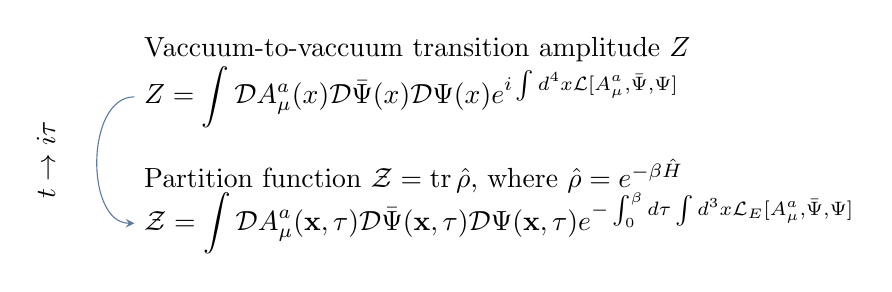
\begin{tikzpicture}
        \node (lb1) at (current page.center) {Vaccuum-to-vaccuum transition amplitude $Z$};
        \node[below=4ex of lb1.west, anchor=west] (eq1) {$\displaystyle Z = \int \mathcal{D} A_\mu^a(x)\mathcal{D}\bar{\Psi}(x)\mathcal{D}\Psi(x)e^{i\int d^4x \mathcal{L}[A_\mu^a,\bar\Psi, \Psi]}$};
        \node[below=1cm of eq1.west, anchor=west] (lb2) {Partition function $\mathcal{Z} = \mathrm{tr}\, \hat{\rho}$, where $\hat{\rho} = e^{-\beta \hat{H}}$};
        \node[below=4ex of lb2.west, anchor=west] (eq2) {$\displaystyle \mathcal{Z} = \int \mathcal{D} A_\mu^a({\bf x}, \tau)\mathcal{D}\bar{\Psi}({\bf x}, \tau)\mathcal{D}\Psi({\bf x}, \tau)e^{-\int_0^\beta d\tau \int d^3x \mathcal{L}_E[A_\mu^a,\bar\Psi, \Psi]}$};
        \path[->, >=stealth, theme] (eq1.west) edge [out=180, in=-180] (eq2.west);
        \node[xshift=-5.2cm, rotate=90] (imag) at ($(eq1)!0.5!(eq2)$) {$t\rightarrow i \tau$}; 
    \end{tikzpicture}
    \begin{columns}[T]
        \begin{column}{0.1\textwidth}
        \end{column}
        \begin{column}{0.33\textwidth}
            Path integral is discretized\\ and solved on a lattice $\rightarrow$ \\[2ex]
            Partition function yields\\ the QCD equation of state
        \end{column}
        \begin{column}{0.3\textwidth}
            \vspace{-.3cm} 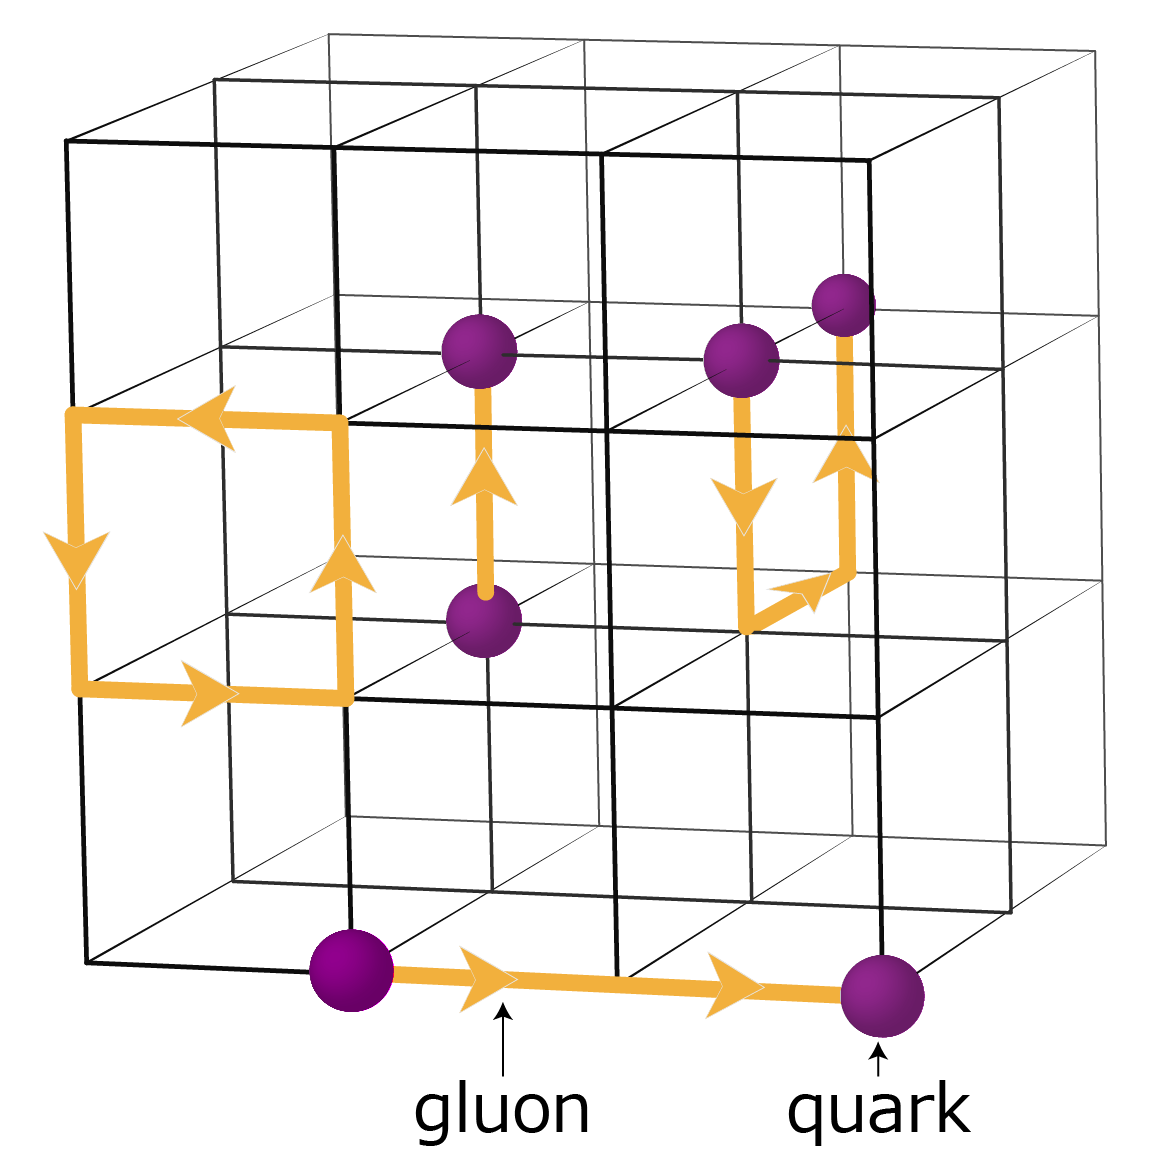
\includegraphics[width=.7\textwidth]{lattice}
        \end{column}
        \begin{column}{0.1\textwidth}
        \end{column}
    \end{columns}
\end{frame}


\begin{frame}[t,plain]{Lattice QCD equation of state error analysis}
    \vspace{0.6cm}
    \begin{columns}[t]
        \begin{column}{0.025\textwidth}
        \end{column}
        \begin{column}{0.575\textwidth}
            {\small Quantify effect of different LQCD equation of state 
                   calculations on heavy-ion collision observables}\\
            \smallskip
            {\scriptsize JSM and RAS, Phys.\ Rev.\ C93, 044913 (2016)}
            \smallskip
            \begin{itemize}
                \small
                \item Three different LQCD EoS calc.
                \item Modern Monte Carlo hydro model
                \item Large scale simulation on open science grid
            \end{itemize}
            \medskip
            \begin{tikzpicture}
                \node at (3.,-1.4) {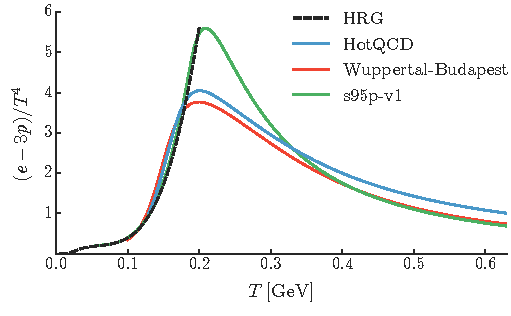
\includegraphics[width=0.7\linewidth]{trace}};
                \tikz[remember picture] \node[coordinate, above=2cm, right=5cm] (d1) {};
            \end{tikzpicture}
        \end{column}
        \begin{column}{0.4\textwidth}
            \bigskip
            \begin{tikzpicture}
                \node at (2.2,-3.2) {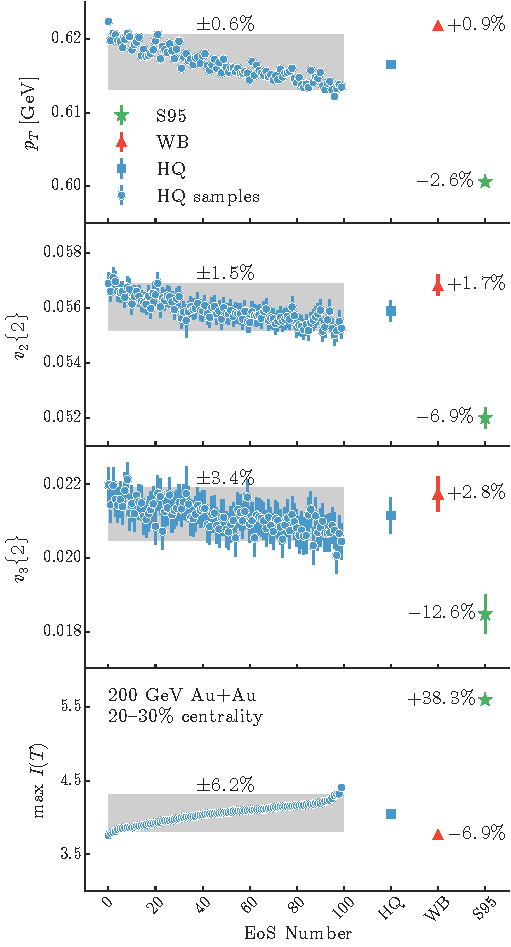
\includegraphics[height=0.8\textheight]{eos_compare}};
                \tikz[remember picture] \node[coordinate, below=4cm, left=.2cm] (d2) {};
            \end{tikzpicture}
        \end{column}
    \end{columns}
    \only<2>{
    \begin{tikzpicture}[remember picture, overlay]
        \path[->, >=stealth, pyred] (d1) edge [out=40, in=-180] ([yshift=-0.6cm]d2);
        \path[->, >=stealth, pyred] (d1) edge [out=40, in=-180] ([yshift=-2.4cm]d2);
        \path[->, >=stealth, pyred] (d1) edge [out=40, in=-180] ([yshift=-4.4cm]d2);
    \end{tikzpicture}}
\end{frame}


\begin{frame}{Current practicum and thesis work}
    \hspace{2cm} \medskip
    \emph{\quad "What are you doing and why are you doing it." \\ \hspace{9.5 cm}--sponsors}
    \bigskip
    \setbeamercovered{transparent}
    \begin{columns}
    \begin{column}{0.8\textwidth}
    \begin{enumerate}
        \onslide<0>{\item Quantify sensitivity of hydrodynamic simulations to different\\ 
              calculations of the QCD equation of state (LLNL)\\
              {\scriptsize Phys.\ Rev.\ C93 (2016) 044913}\\[1ex]}
        \onslide<1>{\item Improve theoretical description of the QGP initial conditions\\
              {\scriptsize Nucl.\ Phys.\ A 904-905, 815c (2013)}\\
              {\scriptsize Phys.\ Rev.\ C92 (2015) 011901}\\[1ex]}
        \onslide<0>{\item Rigorously constrain QGP medium properties using\\ Bayesian model-to-data analysis\\
              {\scriptsize pre-print\, arXiv:1605.03954 (2016)}}
    \end{enumerate}
    \end{column}
    \end{columns}
\end{frame}


\begin{frame}[plain]{What are the initial conditions?}
    \vspace{0.6 cm}
    \small Initial conditions: energy density and fluid velocity at $\tau=\tau_0$.
    \begin{figure}
        \scriptsize Initial energy density (3D)\\
        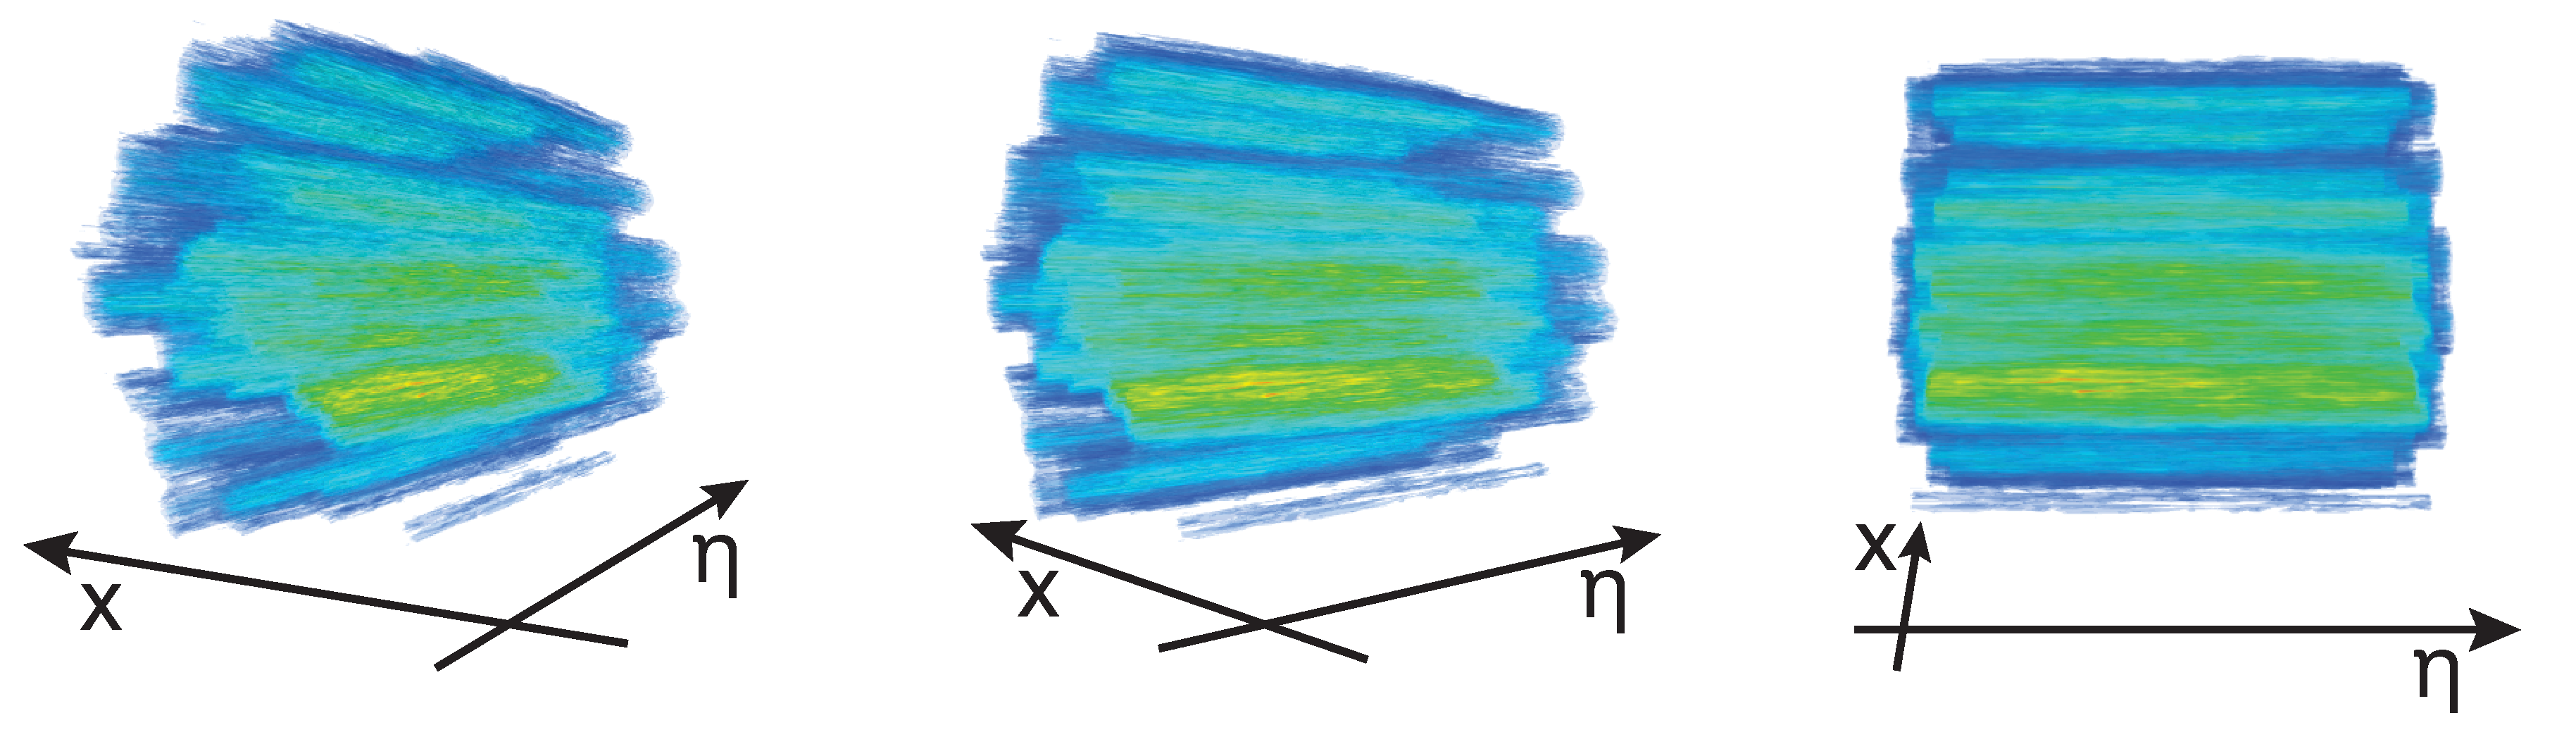
\includegraphics[width=0.55\textwidth]{three_dim}\\
        Figure credit: Schenke, Schlichting
    \end{figure}
    \small Common to project out beam dimension ($\eta$-coordinate)\\
    \begin{figure}
        \scriptsize Initial energy density (2D)\\
        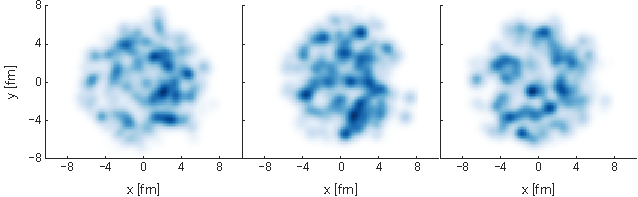
\includegraphics[width=0.6\textwidth]{trento2d}
    \end{figure}
\end{frame}


\begin{frame}[t]{The initial condition problem}
    \vspace{0.6 cm}
    \only<1>{
    \begin{columns}
        \begin{column}{0.025\textwidth}
        \end{column}
        \begin{column}{0.55\textwidth}
            \begin{tcolorbox}[colback=theme!10, colframe=theme!0]
                The QGP initial conditions are\\ 
                \underline{not well understood.} Many models/theories
                proposed in the literature.
            \end{tcolorbox}
        \end{column}
        \begin{column}{0.4\textwidth}
            \centering
            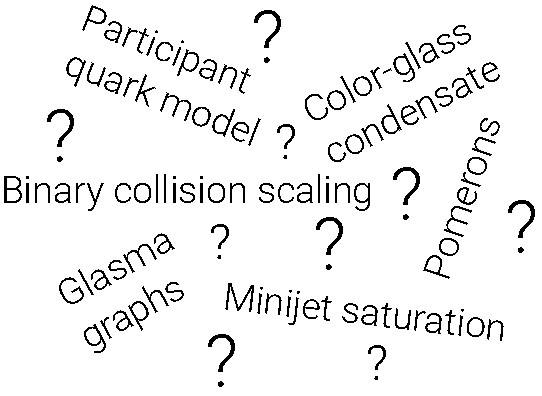
\includegraphics[width=0.65\textwidth]{models}
        \end{column}
        \begin{column}{0.025\textwidth}
        \end{column}
    \end{columns}
    \smallskip
    \begin{itemize}
        \item QGP viscosity extracted by tuning simulation viscosity to fit elliptic flow data.\\[1ex]
        \item \emph{Different} initial condition models predict \emph{different} flow behavior and hence prefer 
              \emph{different} QGP viscosity values!
    \end{itemize}
    \begin{tcolorbox}[colback=pyred!10, colframe=theme!0]
        \centering
        Extracted QGP viscosity depends on theoretical initial conditions!\\[1ex]
        Estimates inherit large theory uncertainty!
    \end{tcolorbox}}
    \only<2>{
        \vspace{1.6 cm}
        \begin{columns}
        \begin{column}{0.8\textwidth}
        \begin{block}{\Large Solution---data driven approach}
            Parametrize QGP initial conditions using flexible 'meta-model'.\\
            Apply rigorous statistical methods to simultaneously constrain initial condition and QGP medium parameters.
        \end{block}
        \end{column}
        \end{columns}
    }
\end{frame}


\begin{frame}{\protect\trento: new parametric initial condition model}
    \only<1>{
    \begin{tikzpicture}[remember picture,overlay]
        \node[anchor=center, xshift=-2 cm, yshift=0.5 cm] at (current page.center) {
            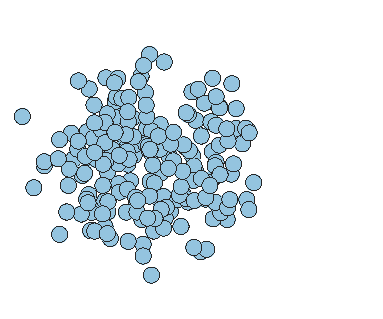
\includegraphics[scale=1]{nucleusB}};
        \node[anchor=center, xshift= 2 cm, yshift=0.5 cm] at (current page.center) {
            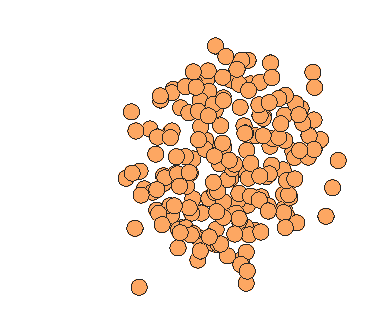
\includegraphics[scale=1]{nucleusA}};
        \node[below = 3cm of current page.center, anchor=center]{
            \centering Sample positions of nucleons within colliding nuclei};
    \end{tikzpicture}}
   
    \only<2>{ 
    \begin{tikzpicture}[remember picture,overlay]
        \node[anchor=center, yshift=0.5 cm] at (current page.center) {
            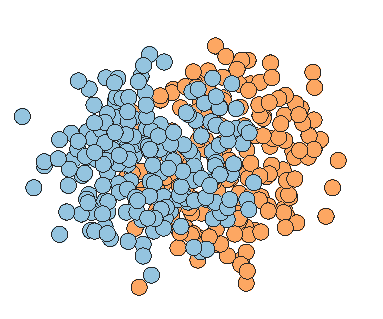
\includegraphics[scale=1]{nucleusAB}};
        \node[below = 3cm of current page.center, anchor=center]{
            \centering Nuclei collide at some random offset (impact parameter)};
    \end{tikzpicture}}
    
    \only<3>{ 
    \begin{tikzpicture}[remember picture,overlay]
        \node[anchor=center, yshift=0.5 cm] at (current page.center) {
            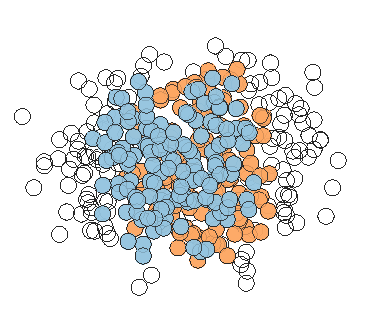
\includegraphics[scale=1]{partAB}};
        \node[below = 3cm of current page.center, anchor=center]{
            \centering Determine nucleons which are struck in the collision};
    \end{tikzpicture}}
    
    \only<4>{
    \begin{tikzpicture}[remember picture,overlay]
        \node[anchor=center, xshift=-2 cm, yshift=0.5 cm] at (current page.center) {
            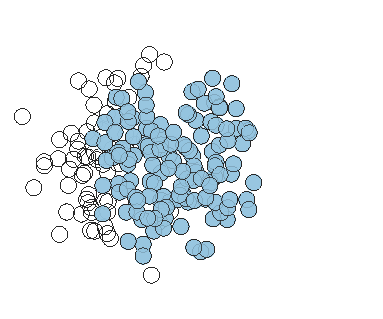
\includegraphics[scale=1]{partB}};
        \node[anchor=center, xshift= 2 cm, yshift=0.5 cm] at (current page.center) {
            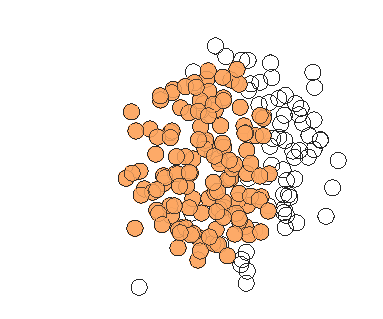
\includegraphics[scale=1]{partA}};
    \end{tikzpicture}}
    
    \only<5>{
    \begin{tikzpicture}[remember picture,overlay]
        \node[anchor=center, xshift=-2 cm, yshift=0.5 cm] at (current page.center) {
            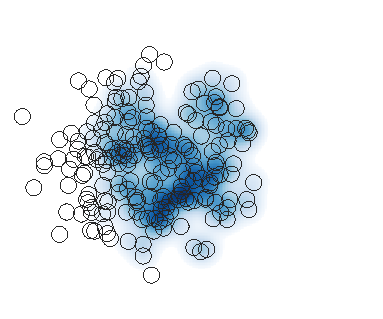
\includegraphics[scale=1]{thickB}};
        \node[anchor=center, xshift= 2 cm, yshift=0.5 cm] at (current page.center) {
            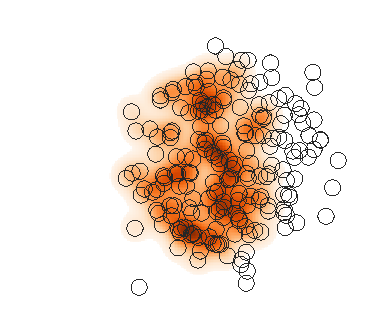
\includegraphics[scale=1]{thickA}};
        \node[below = 3cm of current page.center, anchor=center]{
            \centering Construct participant density---superposition of struck nucleons};
    \end{tikzpicture}}
    
    \only<6>{
    \begin{tikzpicture}[remember picture,overlay]
        \node[anchor=center, yshift=0.5 cm] at (current page.center) {
            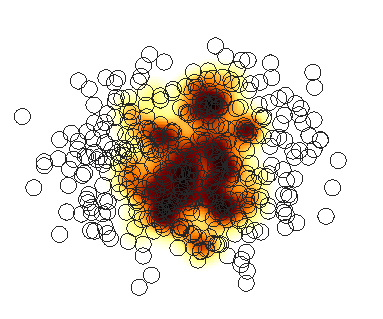
\includegraphics[scale=1]{entropy}};
        \node[below = 3cm of current page.center, align=center, anchor=center]{
            Convert local overlap density $\rightarrow$ entropy deposition\\
            Mapping represents some scalar function of two arguments
        };
    \end{tikzpicture}}
    
\end{frame}


\begin{frame}{Parametrizing local entropy deposition}
    \centering \bigskip
    \begin{columns}
    \begin{column}{0.75\textwidth}
    \centering
    \begin{tcolorbox}[colback=theme!10, colframe=theme!0]
        \centering Generalized mean ansatz: \quad
                   $\displaystyle \frac{dS}{d^2r\, dy} \propto
                    \biggl(\frac{T_A^p + T_B^p}{2}\biggr)^{1/p}$
            \tikz[remember picture] \node[coordinate, above=5 pt] (d1) {};
    \end{tcolorbox}
    \end{column}
    \end{columns}
    \bigskip
    \begin{columns}[T]
        \begin{column}{0.1\textwidth}
        \end{column}
        \begin{column}{0.6\textwidth}
            \centering
            \includegraphics<1>[width=\textwidth]{thickness_band} 
            \includegraphics<2>[width=\textwidth]{thickness_arithmetic} 
            \includegraphics<3>[width=\textwidth]{thickness_geometric} 
            \includegraphics<4>[width=\textwidth]{thickness_harmonic} 
        \end{column}
        \begin{column}{0.25\textwidth}
            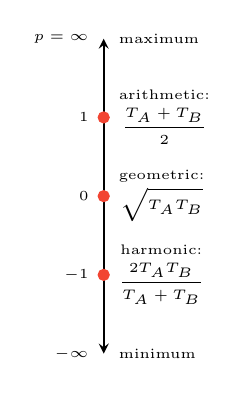
\begin{tikzpicture}
                \tiny
                \tikz[remember picture] \node[coordinate, left=5pt, above=5pt] (d2) {};
                \draw[semithick, <->, >=stealth] (0,0) -- (0,-4);
                \foreach \y in {-1,-2,-3} \draw[semithick] (-2pt, \y cm) -- (2pt, \y cm);
                \draw (0,0) node[left=3pt] {$p=\infty$} node[right=3pt] {maximum};
                \draw (0,-1) node[left=3pt] {$1$} node[right=3pt, align=center] {
                    arithmetic:\\[1ex] $\displaystyle \frac{T_A+T_B}{2}$};
                \draw (0,-2) node[left=3pt] {$0$} node[right=3pt, align=center] {
                    geometric:\\[.4ex] $\displaystyle \sqrt{T_A T_B}$};
                \draw (0,-3) node[left=3pt] {$-1$} node[right=3pt, align=center] {
                    harmonic:\\[1ex] $\displaystyle \frac{2 T_A T_B}{T_A + T_B}$};
                \draw (0,-4) node[left=3pt] {$-\infty$} node[right=3pt] {minimum};
                \draw<2>[pyred, fill=pyred] (0,-1) circle (2 pt);
                \draw<3>[pyred, fill=pyred] (0,-2) circle (2 pt);
                \draw<4>[pyred, fill=pyred] (0,-3) circle (2 pt);
            \end{tikzpicture} 
        \end{column}
        \begin{column}{0.05\textwidth}
        \end{column}
    \end{columns}

    \begin{tikzpicture}[remember picture, overlay]
        \path[->, >=stealth, theme] (d1) edge [out=-45, in=45] (d2);
    \end{tikzpicture}
\end{frame}


\begin{frame}[t]{Compare parametrization to existing IC models}
    \medskip
    \begin{columns}[T]
        \begin{column}{0.1\textwidth}
        \end{column}
        \begin{column}{0.3\textwidth}
            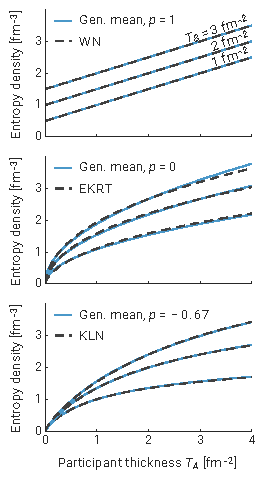
\includegraphics[height=0.8\textheight]{cgc_compare}
        \end{column}
        \begin{column}{0.6\textwidth}
            \begin{itemize}
                \itemsep2ex \small
                \item Wounded nucleon model \\[1em]
                      $\displaystyle \frac{dS}{dy\,d^2r_\perp} 
                      \propto T_A + T_B$ \\[1em]
                      {\scriptsize $^*T$ denotes \emph{participant} thickness} 
                \item EKRT model \; {\scriptsize \color{theme} 
                      PRC 93, 024907 (2016)} \\
                      {\scriptsize after brief free streaming phase} \\[1em] 
                      $\displaystyle \frac{dE_T}{dy\,d^2r_\perp}  \sim 
                      \frac{K_\text{sat}}{\pi} p_\text{sat}^3(K_\text{sat}, 
                      \beta; T_A, T_B)$
                \item KLN model \; {\scriptsize \color{theme} PRC 75, 
                     034905 (2007)} \\[1em] $\displaystyle 
                     \frac{dN_g}{dy\,d^2r_\perp} \sim Q^2_{s,\text{min}} \bigg[2 + 
                     \log \bigg(\frac{Q^2_{s,\text{max}}}{Q^2_{s,\text{min}}}
                     \bigg) \bigg]$
            \end{itemize}
        \end{column}
    \end{columns}
\end{frame}


\begin{frame}{Modern event-by-event hybrid model}
    \smallskip
    \begin{columns}
    \begin{column}{0.05\textwidth}
    \end{column}
    \begin{column}{0.95\textwidth}
    \begin{itemize}
        \item \trento\ initial conditions \\
        {\scriptsize Moreland, Bernhard, Bass, PRC {\bf 92}, 
         no.\ 1, 011901 (2015)} \\
        \begin{table}
            \scriptsize \flushleft
            \begin{tabular}{r l}
                norm & entropy normalization \\ 
                $p$ & entropy deposition parameter \\
                $k$ & proton-proton multiplicity fluctuations \\
                $w$ & Gaussian nucleon width
            \end{tabular}
        \end{table}
        \smallskip
        \item HotQCD equation of state \\
        {\scriptsize Bazavov, et.\ al.\ PRD {\bf 90}, 
         094503 (2014)} \\
        \smallskip 
        \item iEBE-VISHNU hydrodynamics \\
        {\scriptsize Shen, Qiu, Song, Bernhard, Bass, Heinz, 
         Comp.\ Phys.\ Comm.\ {\bf 199}, 61 (2016)}  
        \begin{table}
            \scriptsize \flushleft
            \begin{tabular}{r l}
                $\eta/s$ min & shear viscosity minimum \\ 
                $\eta/s$ slope & shear viscosity slope \\
                $\zeta/s$ norm & bulk viscosity normalization \\
                $T_\text{sw}$ & hydro-to-urqmd switching temp
            \end{tabular}
        \end{table}
        \smallskip
        \item UrQMD hadronic afterburner \\
        {\scriptsize Bass et.\ al, Prog.\ Part.\ Nucl.\ Phys.\ 
         {\bf 41}, 255 (1998)}
    \end{itemize}
    \end{column}
    \end{columns}
\end{frame}


\begin{frame}{The challenge of rigorous model-to-data comparison}
    \begin{tikzpicture}[overlay, remember picture]
        \node [anchor=east, left=1cm  of current page.north, yshift=-1.8cm] 
            (t1) {\large Parameter};
        \node [anchor=west, right=1cm of current page.north, yshift=-1.8cm] 
            (t2) {\large Observable};
        \node [anchor=east, left=1cm  of current page.north, yshift=-2.4cm] 
            (a1) {\small shear viscosity};
        \node [anchor=east, left=1cm  of current page.north, yshift=-2.9cm] 
            (a2) {\small bulk viscosity};
        \node [anchor=east, left=1cm  of current page.north, yshift=-3.4cm] 
            (a3) {\small pre-equilibrium flow};
        \node [anchor=east, left=1cm  of current page.north, yshift=-3.9cm] 
            (a4) {\small nucleon width};
        \node [anchor=east, left=1cm  of current page.north, yshift=-4.4cm] 
            (a5) {\small hadronization temp};
        \node [anchor=east, left=1cm  of current page.north, yshift=-4.9cm] 
            (a6) {\small p+p fluctuations};
        \node [anchor=west, right=1cm of current page.north, yshift=-2.4cm] 
            (b1) {\small identified yields};
        \node [anchor=west, right=1cm of current page.north, yshift=-2.9cm] 
            (b2) {\small identified mean $p_T$};
        \node [anchor=west, right=1cm of current page.north, yshift=-3.4cm] 
            (b3) {\small flow cumulants};
        \node [anchor=west, right=1cm of current page.north, yshift=-3.9cm] 
            (b4) {\small mode mixing observables};
        \node [anchor=west, right=1cm of current page.north, yshift=-4.4cm] 
            (b5) {\small event plane decorrelations};
        \node [anchor=west, right=1cm of current page.north, yshift=-4.9cm] 
            (b6) {\small HBT interferometry};

        \draw [almostblack, line width=0.2pt] (a1.east) -- (b1.west);
        \draw [almostblack, line width=0.2pt] (a1.east) -- (b2.west);
        \draw [almostblack, line width=0.2pt] (a1.east) -- (b3.west);
        \draw [almostblack, line width=0.2pt] (a1.east) -- (b4.west);
        \draw [almostblack, line width=0.2pt] (a1.east) -- (b5.west);
        \draw [almostblack, line width=0.2pt] (a1.east) -- (b6.west);
        
        \draw [almostblack, line width=0.2pt] (a2.east) -- (b1.west);
        \draw [almostblack, line width=0.2pt] (a2.east) -- (b2.west);
        \draw [almostblack, line width=0.2pt] (a2.east) -- (b3.west);
        \draw [almostblack, line width=0.2pt] (a2.east) -- (b4.west);
        \draw [almostblack, line width=0.2pt] (a2.east) -- (b5.west);
        \draw [almostblack, line width=0.2pt] (a2.east) -- (b6.west);
        
        \draw [almostblack, line width=0.2pt] (a3.east) -- (b1.west);
        \draw [almostblack, line width=0.2pt] (a3.east) -- (b2.west);
        \draw [almostblack, line width=0.2pt] (a3.east) -- (b3.west);
        \draw [almostblack, line width=0.2pt] (a3.east) -- (b4.west);
        \draw [almostblack, line width=0.2pt] (a3.east) -- (b5.west);
        \draw [almostblack, line width=0.2pt] (a3.east) -- (b6.west);

        \draw [almostblack, line width=0.2pt] (a4.east) -- (b1.west);
        \draw [almostblack, line width=0.2pt] (a4.east) -- (b2.west);
        \draw [almostblack, line width=0.2pt] (a4.east) -- (b3.west);
        \draw [almostblack, line width=0.2pt] (a4.east) -- (b4.west);
        \draw [almostblack, line width=0.2pt] (a4.east) -- (b5.west);
        \draw [almostblack, line width=0.2pt] (a4.east) -- (b6.west);

        \draw [almostblack, line width=0.2pt] (a5.east) -- (b1.west);
        \draw [almostblack, line width=0.2pt] (a5.east) -- (b2.west);
        \draw [almostblack, line width=0.2pt] (a5.east) -- (b3.west);
        \draw [almostblack, line width=0.2pt] (a5.east) -- (b4.west);
        \draw [almostblack, line width=0.2pt] (a5.east) -- (b5.west);
        \draw [almostblack, line width=0.2pt] (a5.east) -- (b6.west);
        
        \draw [almostblack, line width=0.2pt] (a6.east) -- (b1.west);
        \draw [almostblack, line width=0.2pt] (a6.east) -- (b2.west);
        \draw [almostblack, line width=0.2pt] (a6.east) -- (b3.west);
        \draw [almostblack, line width=0.2pt] (a6.east) -- (b4.west);
        \draw [almostblack, line width=0.2pt] (a6.east) -- (b5.west);
        \draw [almostblack, line width=0.2pt] (a6.east) -- (b6.west);
    \end{tikzpicture}
    \vspace{4 cm} \\
    \begin{columns}
    \begin{column}{0.85\textwidth}
    \begin{tcolorbox}[width=\textwidth, colback=theme!10, colframe=theme!0]
        \centering
        \small Testing a single set of parameters requires 
               $\mathcal{O}(10^4)$ hydro events \\
        \small \smallskip ...and evaluating eight different parameters 
               five times each\\ requires $5^8 \times 10^4 \approx 10^9$ 
               hydro events. \bigskip \\
        {\large That's roughly $10^5$ computer \emph{years}!}
    \end{tcolorbox}
    \end{column}
    \end{columns}
\end{frame}


\begin{frame}{Current practicum and thesis work}
    \hspace{2cm} \medskip
    \emph{\quad "What are you doing and why are you doing it." \\ \hspace{9.5 cm}--sponsors}
    \bigskip
    \setbeamercovered{transparent}
    \begin{columns}
    \begin{column}{0.8\textwidth}
    \begin{enumerate}
        \onslide<0>{\item Quantify sensitivity of hydrodynamic simulations to different\\ 
              calculations of the QCD equation of state (LLNL)\\
              {\scriptsize Phys.\ Rev.\ C93 (2016) 044913}\\[1ex]}
        \onslide<0>{\item Improve theoretical description of the QGP initial conditions\\
              {\scriptsize Nucl.\ Phys.\ A 904-905, 815c (2013)}\\
              {\scriptsize Phys.\ Rev.\ C92 (2015) 011901}\\[1ex]}
        \onslide<1>{\item Rigorously constrain QGP medium properties using\\ Bayesian model-to-data analysis\\
              {\scriptsize pre-print\, arXiv:1605.03954 (2016)}}
    \end{enumerate}
    \end{column}
    \end{columns}
\end{frame}


\begin{frame}{Solution: Bayesian methodology}
    \vspace{0.8 cm}
    \centering
    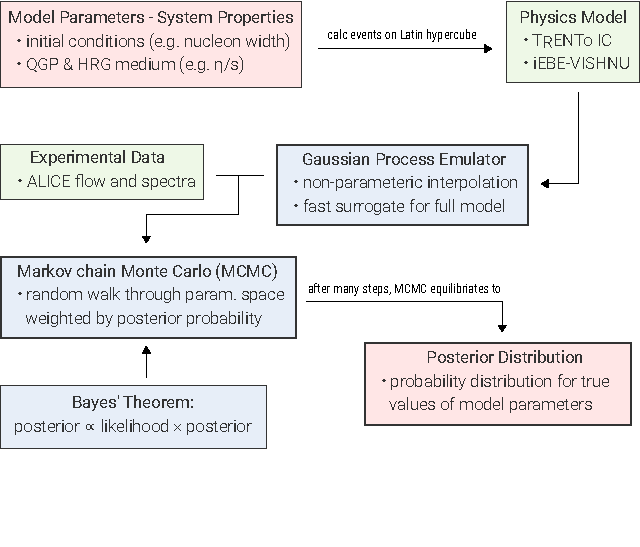
\includegraphics[height=0.95\textheight]{flowchart}
\end{frame}


\begin{frame}{Calibrating the model: before and after}
    \medskip \centering
    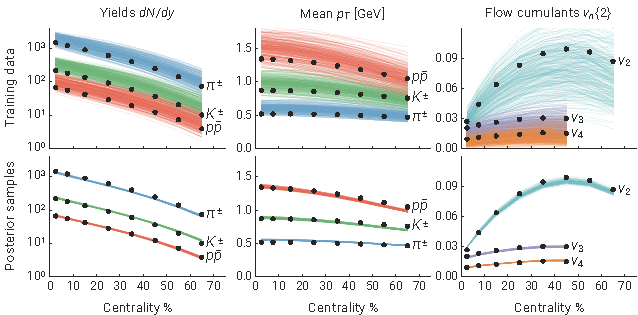
\includegraphics{observables_plot} \\
    \bigskip
    \begin{columns}
    \begin{column}{0.8\textwidth}
    \begin{itemize}
        \small
        \item Top: run model ($\times 10^4$ events) at each design 
              point ($\times300$ evals)
        \vspace{0.2 cm}
        \item Bottom: emulator predictions for 100 samples from 
              the posterior
    \end{itemize}
    \end{column}
    \end{columns}
\end{frame}


\begin{frame}[plain]
    \begin{columns}
        \begin{column}{1 cm}
            \centering
            \hspace{0.5 cm}
            \rotatebox[origin=c]{90}{
                \scriptsize \only<1>{\color{pyblue}} 
                \only<2->{\color{pyblue!40}} 
                    Calibrated to identified particles
            }
        \end{column}
        \begin{column}{\paperheight}
            \centering \vspace{0.1cm}
            \begin{tikzpicture}
                \only<1>{\node [opacity=1] (post) {
                    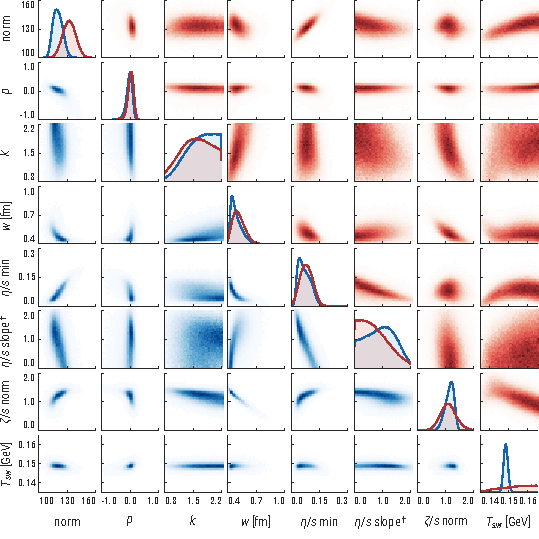
\includegraphics[height=0.98\pageheight]{posterior}};}
                \only<2->{\node [opacity=0.3] (post) {
                    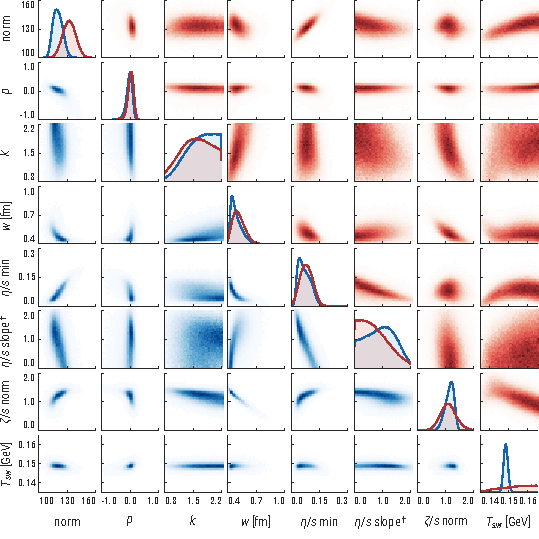
\includegraphics[height=0.98\pageheight]{posterior}};}
            \end{tikzpicture}
        \end{column}
        \begin{column}{1 cm}
            \centering
            \rotatebox[origin=c]{-90}{
                \scriptsize \only<1>{\color{pyred}} 
                \only<2->{\color{pyred!40}} 
                    Calibrated to charged particles
            }
            \hspace{0.4 cm}
        \end{column}
    \end{columns}

    \only<2>{
    \begin{tikzpicture}[remember picture, overlay]
        \filldraw [draw=almostblack, fill=almostblack, overlay, 
                   opacity=0.1, anchor=center] (current page.south west) 
                   rectangle (\pagewidth,\pagewidth);
        \node[inner sep=0pt, yshift=1cm, overlay] (node1) at 
              (current page.center) {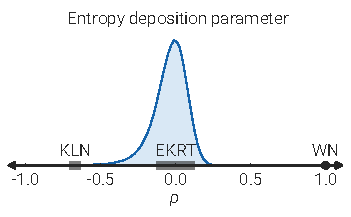
\includegraphics{posterior_p_arrows}};
        \node[inner sep=0pt, below=2ex of node1.south, anchor=north] {
            \begin{tcolorbox}[width=0.424\textwidth, boxrule=0pt, 
                              colback=white, colframe=almostblack, sharp corners]
                \scriptsize \centering
                Generalized mean parametrization: \medskip \\
                $dS/dy \propto \Big(\frac{T_A^p + T_B^p}{2}\Big)^{1/p}$
            \end{tcolorbox}
        };
    \end{tikzpicture}}
    
    \only<3>{
    \begin{tikzpicture}[remember picture, overlay]
        \filldraw [draw=almostblack, fill=almostblack, 
                    overlay, opacity=0.1, 
            anchor=center] (current page.south west) rectangle 
            (\pagewidth,\pagewidth);
        \node[inner sep=0pt, yshift=1cm] at (current page.center) 
            {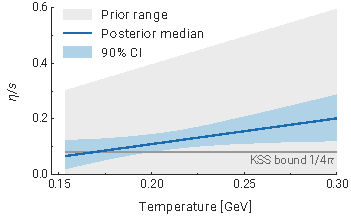
\includegraphics{etas_estimate}};
        \node[inner sep=0pt, below=2ex of node1.south, anchor=north] {
            \begin{tcolorbox}[width=0.424\textwidth, boxrule=0pt, 
                colback=white, colframe=almostblack, sharp corners]
                \scriptsize \centering
                Shear viscosity parametrization: \medskip \\
                $(\eta/s)(T) = (\eta/s)_\text{min} + (T - T_c) 
                (\eta/s)_\text{slope}$ 
            \end{tcolorbox}
        };
    \end{tikzpicture}}
    
\end{frame}


\begin{frame}[t]{Running the model with high probability parameters}
    \centering \vspace{0.4 cm}
    \begin{columns}[T]
        \begin{column}{0.05\textwidth}
        \end{column}
        \begin{column}{0.4\textwidth}
            \scriptsize
            \begin{itemize}
                \item Choose high probability model parameters 
                      from Bayesian\\ posterior (right)
                \smallskip
                \item Run full hybrid model using high probability 
                      parameters (bottom)
            \end{itemize}
        \end{column}
        \begin{column}{0.46\textwidth}
            \scriptsize
            \begin{tabular}{lllll}
                \multicolumn{2}{c}{Initial condition} & & 
                    \multicolumn{2}{c}{QGP medium} \\
                \noalign{\smallskip}\hline\noalign{\medskip}
                norm & 120.          &&  $\eta/s$ min   & 0.08       \\
                $p$  & 0.0           &&  $\eta/s$ slope & 0.85 GeV$^{-1}$   \\
                $k$  & 1.5           &&  $\zeta/s$ norm & 1.25       \\
                $w$  & 0.43 fm       &&  $T_\text{sw}$  & 0.148 GeV  \\
            \end{tabular}
        \end{column}
        \begin{column}{0.05\textwidth}
        \end{column}
    \end{columns}
    \vspace{0.5 cm}
    \only<1>{\centering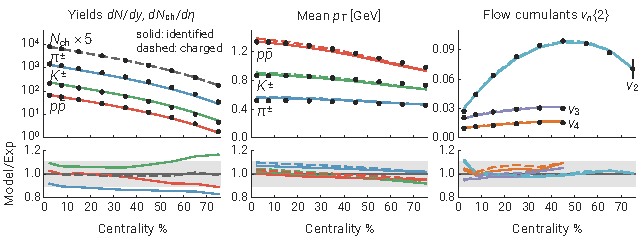
\includegraphics[width=0.85\textwidth]{mode_observables}}
    \only<2>{
        \bigskip
        \begin{columns}[T]
            \begin{column}{0.05\textwidth}
            \end{column}
            \begin{column}{0.51\textwidth}
                \centering
                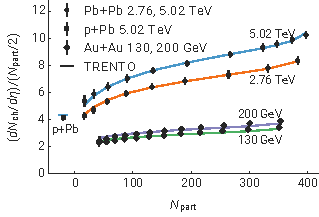
\includegraphics[width=0.9\textwidth]{nch_per_npart}
            \end{column}
            \begin{column}{0.37\textwidth}
                \scriptsize \flushleft
                \begin{itemize}
                    \item Also describes particle production for different 
                    collision systems at multiple beam energies.
                \end{itemize}
            \end{column}
            \begin{column}{0.07\textwidth}
            \end{column}
        \end{columns}
    }
\end{frame}


\begin{frame}[plain]{Conclusions}
    \medskip
    \begin{columns}
    \begin{column}{0.85\textwidth}
        Lattice QCD equation of state (LLNL summer project)
        \begin{itemize}
            \item Modern LQCD equations of state in good agreement.\\ Negligible differences for experimental observables. 
        \end{itemize}
        \smallskip
        Initial condition properties
        \begin{itemize}
            \item Yields, mean $p_T$ and flows impose strong constraints on IC. \\
            \item Entropy  deposition mimicked by $dS/dy \sim \sqrt{T_A T_B}$ \\
            \item Preferred initial conditions agree with two theory calc. \\
        \end{itemize}
        \smallskip
        Hydrodynamic transport properties
        \begin{itemize}
            \item First quantitative credibility interval on $(\eta/s)(T)$!
        \end{itemize}
    \end{column}
    \end{columns}
\end{frame}


\begin{frame}[plain]
    \centering
    \emph{Special thanks to the Krell institute for the exceptional support!}
\end{frame}

\appendix


\begin{frame}{Backup: computer experiment design}
    \begin{columns}
    \begin{column}{0.05\textwidth} 
    \end{column}
    \begin{column}{0.47\textwidth} 
        Maximin Latin hypercube
        \begin{itemize}
            \item Random, space-filling points
            \item \emph{Maximizes} the \emph{minimum}\\
                distance between points\\
                $\rightarrow$ avoids gaps and clusters
            \item Uniform projections into\\
                lower dimensions
        \end{itemize}
        \medskip
        This work:
        \begin{itemize}
            \item 300 points across 8\\
                dimensions
            \item 8 centrality bins
            \item $\mathcal{O}(10^7)$ events total
        \end{itemize}
    \end{column}
    \begin{column}{0.48\textwidth}
        \flushleft 
        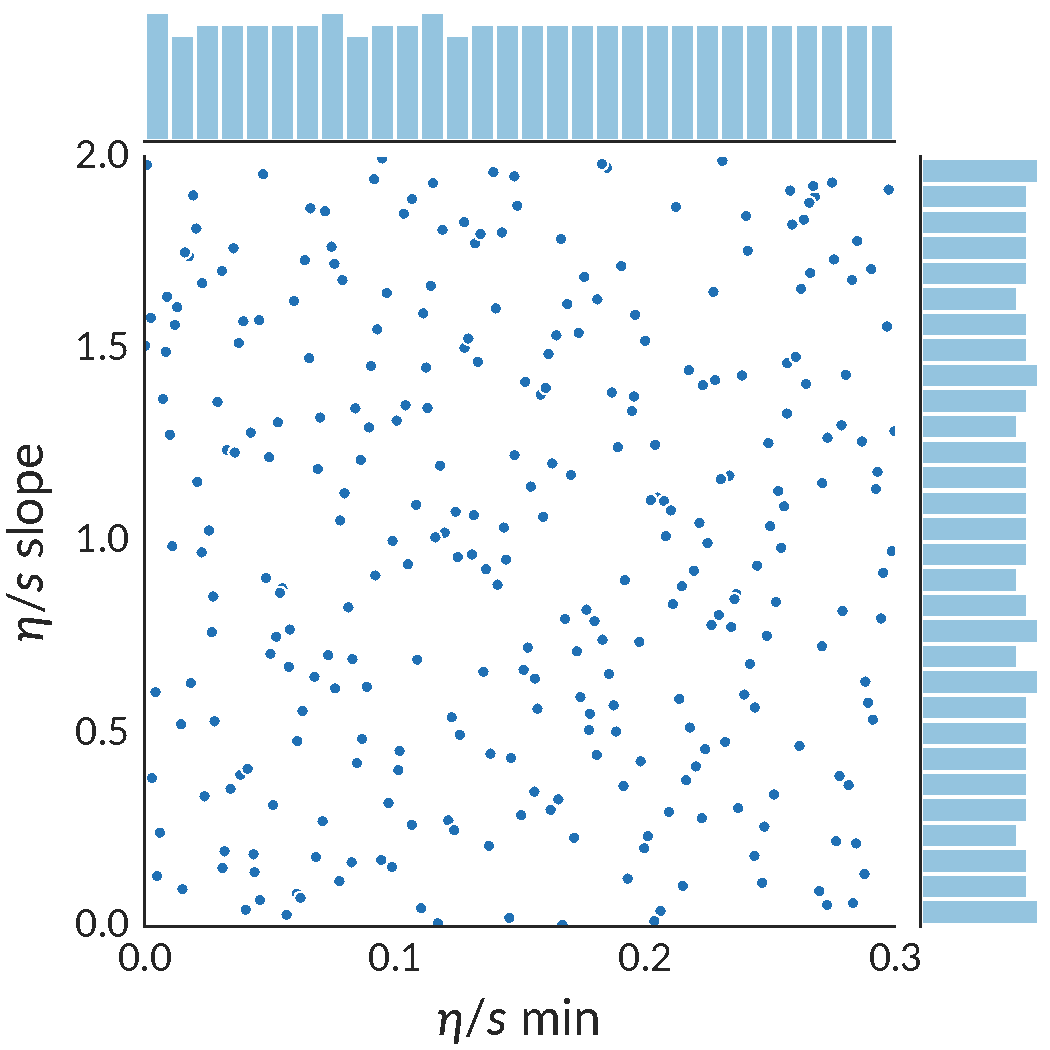
\includegraphics[width=\textwidth]{design}
    \end{column}
    \end{columns}
\end{frame}

\end{document}
